%%%%%%%%%%%%%%%%%%%%%%%%%%%%%%%%%%%%%%%%%%%%%%%%%%%%%%%%%%%%%%%%%%%%%%
%%\documentclass[master]{hdu-thesis}[]中不同的模式选择对应不同的模板%%%%
%|bachelor_p| 本科生毕业设计(论文)模板 | 
%|bachelor_review| 本科生毕设送审(盲审)模板 |
%|master| 学术型硕士模板 | 
%|promaster| 专业学位硕士模板 |
%|doctor| 博士学位模板 |
%|engdoctor| 工程博士学位模板 |
%|master_review| 学术型硕士送审模板 |
%|promaster_review| 专业学位硕士送审模板 |
%|doctor_review|  学术型博士送审模板 |
%|engdoctor_review|  工程博士送审模板 |

%%%%%%%%%%%%%%%%%%%%%%%%%%%%%%%%%%%%%%%%%%%%%%%%%%%%%%%%%%%%%%%%%%%%%%
\documentclass[bachelor_p]{hdu-thesis}

\title{基于python的图像搜索引擎设计}{Image search engine based on Python}
\author{龚健晟}{Gong Jiansheng}%%%%%%作者
\advisor{相成娣\quad 翁立}{Xiang ChengDi Weng Li}%%%%%%指导老师
\school{自动化学院}{School of Automation}%%%%学院
\major{电气工程及其自动化}{}%%%%%%%%%%专业
\authornumber{19062314}{} %%%%%%学号
\authorclass{19060113} %%%%%%%%%班级(本科生填)
\completedate{2023}{5}{}  %%%%%%设计完成时间
\authordirection{}{}%%%%研究方向前者对应中文方向,后者对应英文(研究生填)

\begin{document}


%%%%%%%%%%%%%%%%插入封面%%%%%%%%%%%
\makecover
%%%%%%%%%%%%%%%%插入原创性声明%%%%%%%%%
\makedeclaration

%%%%%%%%%%%%%中文摘要%%%%%%%%%%%%%%
 
\cnabstract

本文介绍了图像搜索引擎的发展历史和发展现状。并介绍了一种基于Python的图像搜索引擎的设计方法。该搜索引擎可以通过输入图像,自动检索并返回与之相似的其他图像。具体来说,该项目使用了卷积神经网络(CNN)提取图像特征,并使用欧式相似度算法计算图像之间的相似度。本文还介绍了如何使用Flask框架和HTML技术实现一个基本的Web界面,使用户可以方便地上传和搜索图像。最后,本文对该搜索引擎进行了测试和评估,并讨论了可能的改进方向。这种基于Python的图像搜索引擎具有广泛的应用前景,例如电子商务、医学影像、农业分析等领域。

\cnkeyword{
  图像搜索引擎;Python;图像特征;卷积神经网络;FLASK}

 
%%%%%%%%%%%%%%%英文摘要%%%%%%%%%%%%
\enabstract

This paper introduces the development history and current status of image search engines.And introduces a design method for an image search engine based on Python. This search engine can automatically retrieve and return similar images by inputting them.
Specifically, the project used Convolutional Neural Networks (CNN) to extract image features and used Euclidean similarity algorithms to calculate the similarity between images. This paper also introduces how to use the Flask framework and HTML technology to implement a basic web interface, allowing users to easily upload and search for images. Finally, this paper tested and evaluated the search engine, and discussed possible improvement directions. This Python based image search engine has broad application prospects, such as e-commerce, medical imaging, agricultural analysis, and other fields.

\enkeyword{Image search engine;Python;Image feature;Convolutional Neural Networks;Flask}
	



% \cnabstract
% \begin{center} 
%   {\sihao\bfseries 热爱生命}\\[3pt]


% \end{center} 
%  \cnkeyword{Latex,}
% % %%%%%%%%%%%%%%%英文摘要%%%%%%%%%%%%
% \enabstract
% % The use of latex in terms of thesis's writing.

% \enkeyword{Latex, }NVIDIA


%%%%%%%%%%%%目录%%%%%%%%%%%
\tableofcontents

%%%%%%%%%%%%%%%%%%%%%%%%
%%%%%%%%%%%%%%正文%%%%%%%%%%%%




\chapter{绪论}
\section{引言}
近年来,随着数字图像的广泛应用和互联网的普及,图片作为视觉信息的重要载体在人们的生活、工作和娱乐中扮演着越来越重要的角色。随之相伴而来的,图像检索技术越来越受到人们的广泛关注和使用。

传统的图像搜索方法通常是基于文本的图像搜索(Text-Based Image Retrieval, TBIR),即用户输入与图片相关联的关键词进行检索。但是由于页面描述不准确、关键词缺失等原因,这种方法往往会出现搜索结果不准确、图片与查询内容不匹配等问题。面对这种情况,基于图像内容的图像搜索(Content-Based Image Retrieval, CBIR)便应运而生。

基于图像内容的图像搜索引擎是通过对图像的特征提取、相似性度量等方法,实现以图搜图等功能。这种方法由于不再依赖于人工的关键词匹配,更加准确和全面地满足了用户对图片搜索需求,同时还节省了一定的人力成本。

然而,传统的特征提取和相似性度量的方法由于存在许多局限性,如降维过程中可能失去一些有用信息、在高纬空间中计算耗时长等缺点,导致检索精度和效率并不能够兼顾。并且在构建基于Python实现的图像搜索引擎时仍会面临诸多挑战。一方面,图像特征的提取与匹配需要消耗大量的硬件计算资源;另一方面,由于图像特征可表示的对象范围极广,如何在尽可能缩小特征库规模的情况下仍然保证检索准确度也是一个非常重要的问题。

为了解决上述问题,本项目采用了基于深度学习算法的方法进行图像搜索。在这种方法中,利用卷积神经网络提取输入图片的特征向量并在数据库中与其他特征向量进行快速匹配,相较于传统方法,相似度计算是在更低维度空间中进行操作的,并且准确性也较高。

本项目旨在设计并实现一个开源、高效、可靠性能良好且便于用户部署的图像搜索引擎,提供给用户快捷、准确的图像检索功能。这将对提升图像检索技术水平,推动数字图像领域的发展具有积极意义。
\section{研究背景与发展}
\subsection{图像搜索引擎的定义}

搜索是指查找特定信息的过程。而搜索引擎是一种软件系统,它通过收集互联网上的信息并建立索引,以便用户可以通过关键词或短语来查找所需信息。简单来说,搜索是一个行为,而搜索引擎是一个工具。搜索需要使用搜索引擎才能实现。图像搜索引擎则是指用户通过输入相关文本描述或图片来获取所需图片的一种软件系统。

\subsection{图像搜索的发展历史}
图像是人类获取和交换信息的重要来源,图像搜索作为一门新兴学科,涉及到人类社会的各个领域。近年来随着技术的飞速发展逐步趋于完善,尤其得益于人工智能等领域的突破性进展。

图像搜索历史较短,但发展速度较快。早在上世纪七十年代末,就有学者提出了基于文本的图像检索。不过在当时,图像集都是较小的,且都是由人工进行文本标注的。随后在九十年代初,学术界又提出了基于内容的图像检索思想。

但是在1990年以前,搜索引擎还没有出现,没有人能够在互联网上进行搜索。而蒙特利尔大学的Alan Emtage实现了最初的搜索引擎, 称为Archie引擎, Archie引擎可以在特定的网络中进行相关的信息检索\citep{search2}。

最早的图像搜索网站是由AltaVista于上世纪九十年代末开发的,用户在搜索引擎中输入文本后网页就会返回相应的图片。早期如LYCOS、AltaVista、Yahoo的图片搜索网站并不是通过处理图片本身来满足用户需求的,而是通过人工给图片加以文本描述或通过图片的上下文,进行文本的配对,从而来选择应该返回的图片。它们以人工分类目录为主,特点是人工分类存放网站的各种目录,用户通过多种方式寻找网站,现在也还有这种方式存在。

\begin{figure}[!htb]
  \centering
  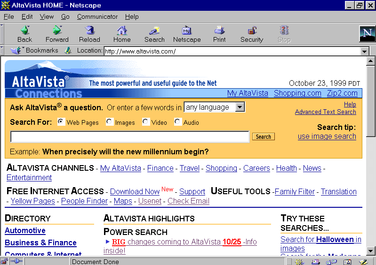
\includegraphics[width=0.5\textwidth]{AltaVista}
  \caption{上世纪九十年代末的AltaVista.}
  \label{fig_AltaVista}
\end{figure}

在2001年,谷歌图像(Google Images)发布,它在短时间内就积累了2.5亿张图片。谷歌图像开发的初衷是因为人们不希望根据网页的上下文来搜索近似图像,而是想要获得他们心中所想的那一张确切图像。这一想法的具体催化剂是2000年的格莱美颁奖仪式,拉丁天后詹妮佛洛佩兹(Jennifer Lopez)身着绿色的范思哲连衣裙轰动了整个时尚圈。节目播出当晚图像搜索网站的搜索量更是增加了数倍。而这同时也反映了早期图像搜索引擎不能满足用户需求的核心原因:用户知道看见了什么,但他们通常不知道要用什么关键词去搜索,尤其是那些具体的人名、地点或物品名等等,通常来说文本的图像搜索无法完美地匹配一张图片。就比如当时的人们直接搜索绿色连衣裙,确实会返回绿色的连衣裙,但绝对不会是他们心中所想的那条。谷歌图像解决这个问题的思路是增加足够多的数据,或许在海量的数据中确实有用户所需要的那些图片,可是用户想要获得他们也绝非易事。

同时期图像标注规模快速的扩大。在2004年前后的社交媒体时代,Flicker上图片的标签也是人为标注的,但是通过广大使用人群,标签总量就变得非常地大,节省了大量的人工成本,以此为基础的图像搜索在小规模数据中有不错的结果和应用前景。但在标注图片过程中,还是会很大程度上受到标注人的主观意识、不同的认知水平所影响,会发生标签文本不匹配的问题。

开发者们由此很快意识到,一个更好的图像搜索必然是基于图像内容即图像本身特征信息的,而不是扫描匹配图像周围的文字。从图片本身获取其特征信息,并与已有数据库中的特征信息进行计算匹配显然会是一种更好的搜索方式。但是基于文本到基于图像内容的图像搜索并没有很快被实现。早期的实验型内容搜索图像引擎数据库集合较小,远不及同时期的谷歌、雅虎,他们的图像搜索引擎约有十亿张图片(截止至2005年)。导致这种情况的原因一方面是当时的硬件性能不足,另一方面是当时并没有一种真正能够“描述”图像的技术。在当时计算机或许能够很好地根据图像的尺寸来分类,但在真正要识别图像内容时,灰域(Grey Areas)出现了。比如说,两张在同一区域内有高对比度的图像有可能会配对,即使他们是完全不同事物的图像。这些因素大大限制了在世纪初CBIR技术的应用,在当时使用CBIR技术的最大的图书馆也仅仅记录了300万张图像,这个数量显然是不足够的。

\begin{figure}[!htb]
  \centering
  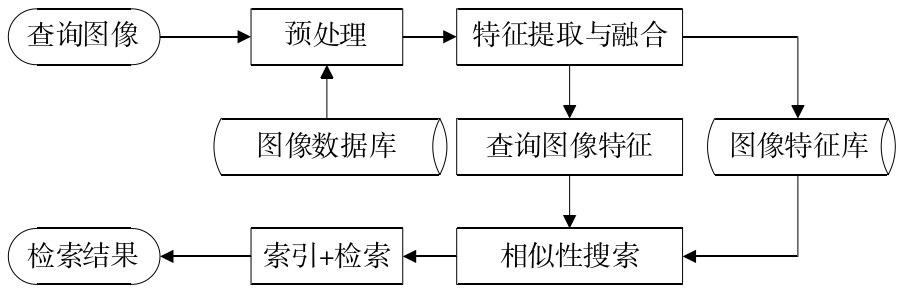
\includegraphics[width=1\textwidth]{CBIR}
  \caption{CBIR一般框架.}
  \label{fig_AltaVista}
\end{figure}

在早期的CBIR实现过程中,当图像搜索的数据库量非常大时,以当时的技术水平和硬件设备是没有办法把用户上传的图像特征与数据库里面的图像进行一一比对匹配的。如果数据库中图像只有几千个或者上万个还是能够满足一些要求的,但这个时候搜索结果又会不尽人意。

2008年,TinEye被推出。TinEye可以非常精确地匹配你要查找的目标图像, 而且搜索速度相当快\citep{TinEye}。同时它也是世界上第一个使用图像到图像的搜索引擎,还很好的解决了上述图像数据库规模过大时会导致响应速度过慢的问题。用户在上传图像后网站会返回该图像的其他版本或高度相似的图片(前提是数据库中有)。它解决数据库过大的思路是把图片进行索引,图像的描述是它的各种特征,而这个特征是一个向量,这个向量怎样能够有效地组织起来实现快速地检索,这是当时TinEye系统往前走了一步的问题。

\begin{figure}[!htb]
  \centering
  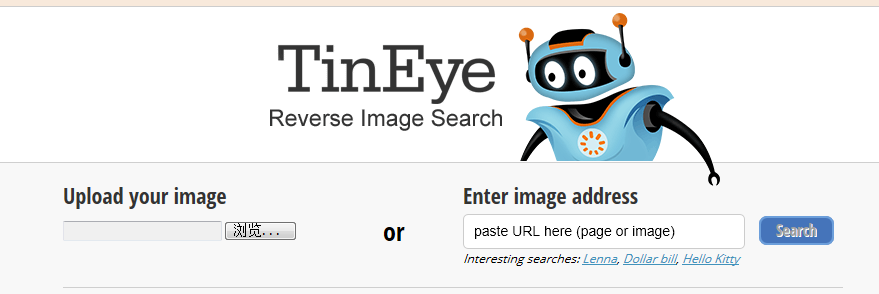
\includegraphics[width=1\textwidth]{tineye}
  \caption{TinEye反向图片搜索网站.}
  \label{fig_tineye}
\end{figure}

TinEye的发布和广泛的使用也昭示着迄今为止最为有效地CBIR形式:“反向”图像搜索的诞生。用户可以直接上传图像进行搜索,而不是使用文本来描述图片,这使得图像搜索时消除了一层猜疑链。用户上传图像后网站会返回该图像的其他版本或高度相似的图片(前提是数据库中有)。 我们今天仍在使用反向搜索,它的功能虽然很强大,但它并没有涵盖图像搜索的所有弱点。如准确率高度依赖数据库的数量和质量,受图像拍摄视角、光影、物体拉伸形变、噪声等等因素影响较大。 

随着视觉属性的图像索引越来越准确,搜索引擎开始实现将相似图片聚集在一起响应搜索的功能。谷歌的Image Swirl就是这样一个项目,也是该公司出于消费者目的而推出研究的首批项目之一。它将寻找视觉线索与照片的文本元素结合起来,让用户可以探索相似的图像。

\subsection{图像搜索引擎中新技术的使用}

在图像搜索引擎不断升级迭代的同时,其他新技术、新理论也被引入到学术界中。例如图形处理器、卷积神经网络等等。

ImageNet项目是一个用于视觉对象识别软件研究的大型可视化数据库。自2010年以来,每年ImageNet都会举办大规模视觉识别挑战赛(ILSVRC,Large Scale Visual Recognition Challenge),研究团队会在给定的数据集上评估其算法,并在几项视觉识别任务中争夺更高的准确性,被誉为图像界的“奥赛”。 \citep{BaiduImageNet}。在2010年和2011年,ImageNet挑战赛的最低差错率分别是29.2$\%$和25.2$\%$,而有的团队差错率甚至高达百分之九十九。2012年,来自多伦多大学的博士生Alex Krizhevsky,用120万张图片训练神经网络模型,和前人不同的是,他选择用英伟达GeForce GPU( GeForce Graphics Processing Unit,英伟达NVIDIA旗下的品牌图形处理器)为训练提供算力。在当年的ImageNet,Krizhevsky的模型以约15$\%$的差错率夺冠,震惊了神经网络学术圈。这个成果得益于GeForce GPU搭载的CUDA(Compute Unified Device Architecture,统一计算架构)平台,能够充分调用显卡的算力、接口,并提供多种工具辅助用户进行开发。

这一标志性事件,证明了GPU对于深度学习的价值,也打破了深度学习的算力枷锁。自此,GPU被广泛应用于AI训练等大规模并发计算场景。数据显示,在2010—2011年,ImageNet挑战赛中没有任何团队使用GPU,2012年Krizhevsky首开先河后,2013年参赛团队使用的GPU达到了60块,2014年进一步提升至110块。

\begin{figure}[!htb]
  \centering
  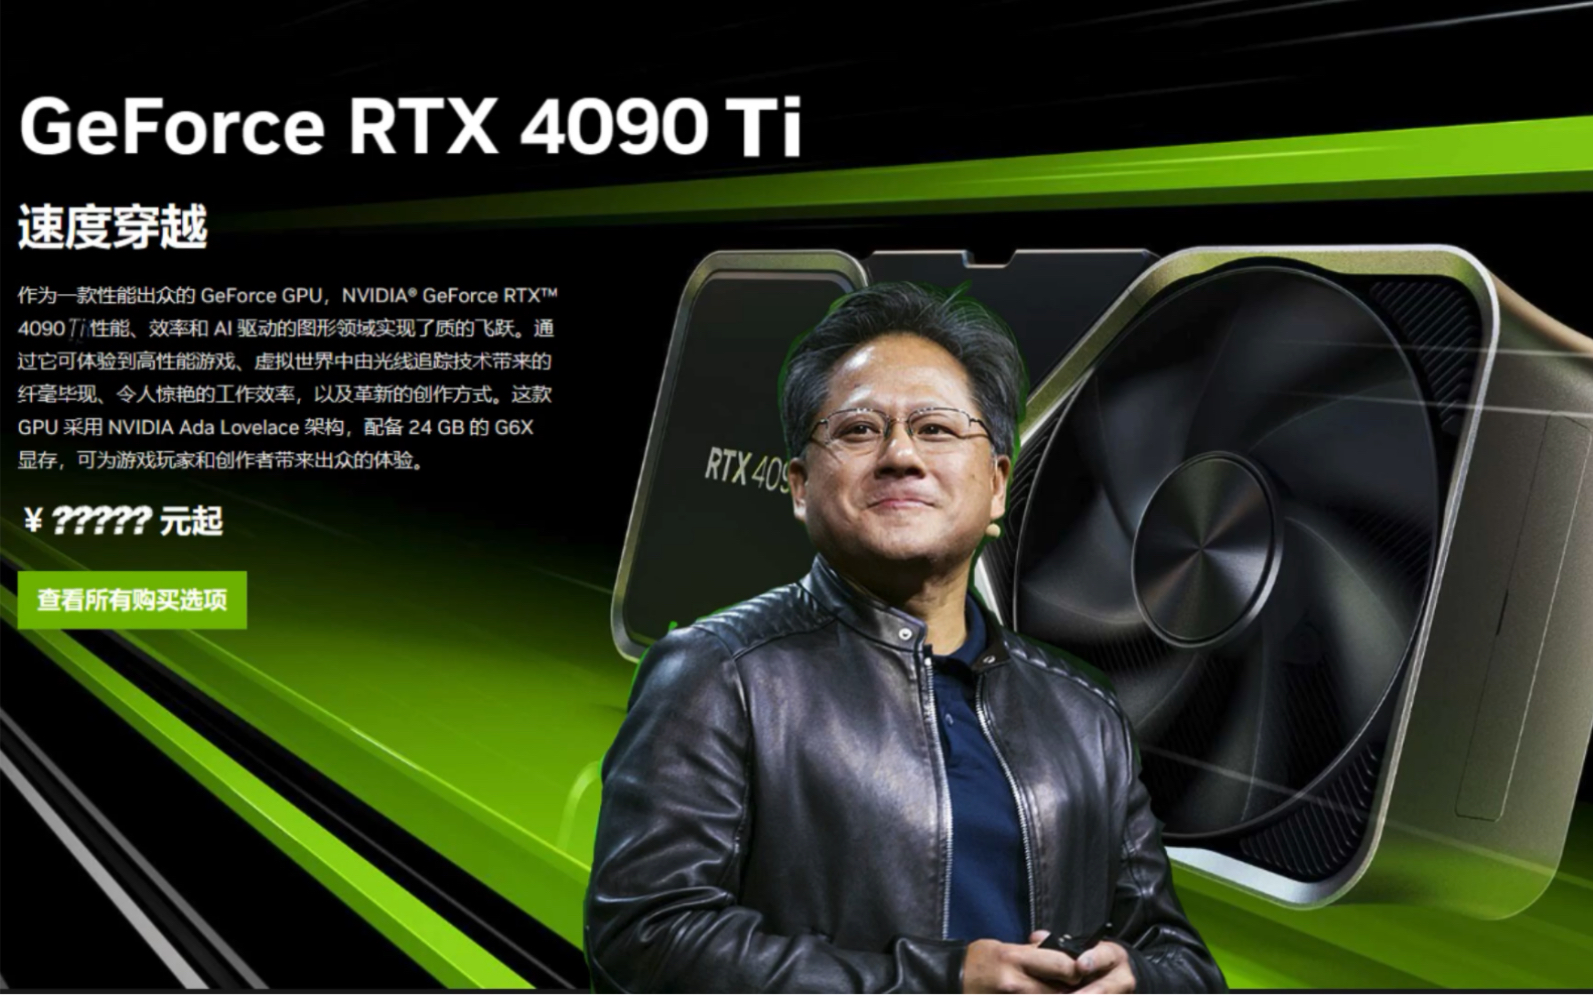
\includegraphics[width=0.85\textwidth]{GPU1}
  \caption{NVIDIA首席执行官黄仁勋与最新款的4090ti,其算力已达1.67个“天网”.}
  \label{fig_GPU1}
\end{figure}

GPU的强大性能在受到各界广泛关注时也在飞速发展着。NVIDIA首席执行官黄仁勋曾在公开场合多次提到英伟达图形处理器的发展速度已经打破了摩尔定律(英特尔创始人之一戈登·摩尔的经验之谈。简短来说就是处理器的性能大约每两年翻一倍,同时价格下降为之前的一半。),GPU性能翻倍所花费的最短时间甚至只要三个月。由于经历了虚拟货币挖矿潮、OpenAI ChatGPT(美国OpenAI旗下的当红AI聊天机器人程序,Chat Generative Pre-trained Transformer)等多个市场显卡需求爆点,深耕于算力、AI与开发者亲和度的英伟达一家企业几乎垄断了当下的GPU市场。无论是消费级显卡还是专业级显卡都能经常见到英伟达的身影,诸多实验室出于经济性考虑也会选择英伟达的消费级显卡来为工作站提供算力。

早期的基于图像内容的图像搜索方法主要是通过人工来提取图像特征, 但是人工提取不仅工作量大而且提取图像特征的准确度也不够高。但随着技术的发展,深度学习近年来逐渐成为热门,我们可以利用深度学习和已有的卷积神经网络(Convolutional Neural Network, CNN)原理, 建立模型让系统自己学习图像的特征, 这样就可以大大降低人工提取特征的误差\citep{CNN1}。CNN是一种前馈神经网络,由一个或多个卷积层、池化层以及顶部的全连接层组成,在图像处理领域表现出色。

卷积神经网络与一般的神经网络的区别在于, 卷积神经网络包含一个由卷积层和次采样层组成的特征抽取器。在卷积神经网络的卷积层中, 一个神经元仅与部分相邻层的神经元连接。在CNN的卷积层,神经元平面分享相同的特征权重.卷积核通常以随机十进制矩阵的形式初始化。在网络的训练过程中, 卷积核将学习获得一个合理的权重。共享权重 (卷积核) 的直接好处是减少网络层之间的连接性,同时减少过拟合的风险.抽样也叫池, 通常用平均抽样 (平均池) 和最大抽样 (MAX池) 两种形式。次采样可以看作是一个特殊的卷积过程。卷积和次采样大大减少了模型的参数, 降低了模型的复杂度\citep{CNN1}。

CNN的卷积运算从频域角度来看,是频谱相乘所以图像跟卷积核做卷积时两者频谱不重叠的部分相乘,结果自然是0,那图像这部分频率的信息就被卷积核过滤了。而图像,本质上就是二维离散的信号,像素点值的大小代表该位置的振幅,所以图像包含了一系列频率的特征。比如图像边缘部分,像素值差别大时属于高频信号,背景部分,像素值差别小时是低频信号。所以如果卷积核具有『高通』性质,就能起到提取图像边缘的作用,低通则有模糊的效果。所以,卷积神经网络的强大之处在于通过卷积层的不同卷积核,提取图像不同频段的特征;以及通过池化层,提取不同粒度的特征\citep{CNN2}。

\begin{figure}[!htb]
  \centering
  \includegraphics[width=0.85\textwidth]{Lenet}
  \caption{早期卷积神经网络LeNet-5结构示意图.}
  \label{fig_LENET}
\end{figure}

卷积神经网络可以提取出图像中的多种特征,这些特征在图像处理、计算机视觉等领域有着广泛的应用。包括但不限于以下几种:
边缘特征:卷积层可以通过滤波器的卷积运算提取图像中的边缘信息。
纹理特征:卷积层可以检测图像中的纹理特征,例如条纹、点等。
形状特征:卷积神经网络可以提取出物体的形状特征,例如圆形、长方形等。
颜色特征:卷积神经网络可以识别图像中的颜色信息,例如红色、绿色等。
统计特征:CNN还可以提取一些统计特征,例如均值、标准差等。
层次特征:深层的卷积层可以提取出更加抽象的特征,例如物体的部件、轮廓等。
时空特征:对于视频等多媒体数据,CNN还可以提取时空特征,例如运动方向、速度等。


\section{国内外研究现状}

目前,国内外的图像搜索引擎研究已经取得了相当的进展。在国外,Google、Bing(必应,微软旗下的搜索网站)等大型搜索引擎公司在图像搜索领域已经取得了很多进展。例如,Google推出了以文本和图像为输入的搜索引擎Google Image Search,并且不断改进其算法和界面。Bing也推出了类似的图像搜索功能,并且支持语义化搜索和人脸识别等高级功能。

在国内,随着互联网应用的快速发展,越来越多的群体开始关注和投入到图像搜索引擎领域。例如,百度推出了百度图片、百度识图等产品,并且不断优化其算法和服务质量。腾讯也推出了基于微信平台的图片搜索功能,并且支持语音输入和智能推荐等特色功能。此外,还有一些企业和高校开展了相关研究工作,如清华大学、中科院自动化所等。

下面将从多个方面论述图像检索的研究现状。

\subsection{传统特征}

当CBIR系统在提取图像特征以表达图像语义时,如何选取合适的特征发挥着至关重要的作用。一般来说我们可以分将传统特征为局部特征和全局特征。其中局部特征通常将图片分割为块或通关计算图像中某些关键点来进行获取;全局特征则描述的是整幅图像。

\subsubsection{全局特征}

传统的的全局特征通常会使用颜色、纹理、形状、空间信息等全局特征,这些特征计算简单且较为直观。

\begin{figure}[!htb]
  \centering
  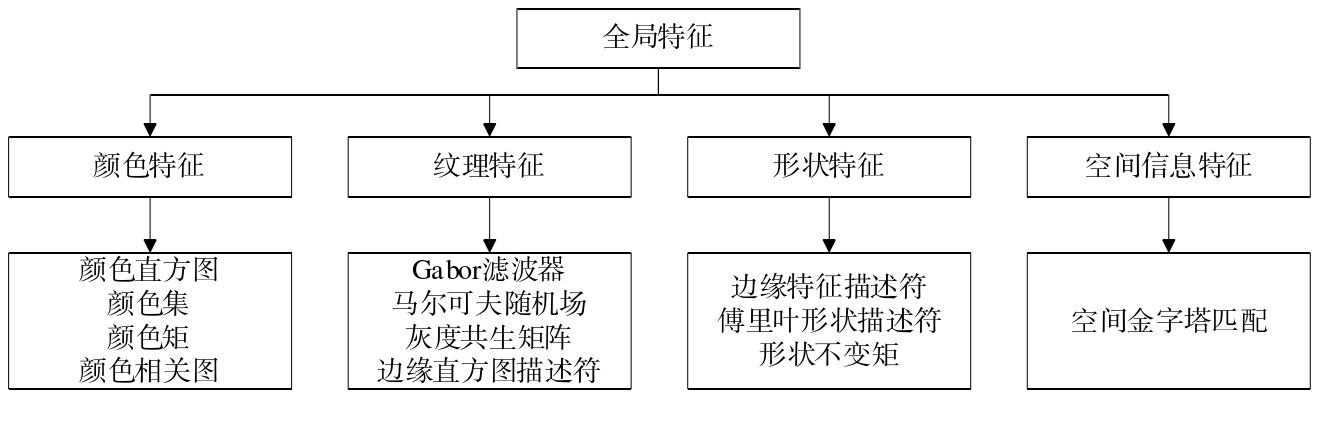
\includegraphics[width=1\textwidth]{FULLIMAGE}
  \caption{全局特征分类及其提取方法.}
  \label{fig_FULLIMAGE}
\end{figure}

颜色特征是图像检索广泛使用的一种直观特征。研究者们根据颜色空间计算颜色特诊,在CBIR领域中最常用的颜色空间包括RGB、HSV、YCvCr、LAB和YUV。这些颜色空间可以用用颜色直方图(CH)、颜色集、颜色矩、颜色相关图等描述符进行表示\citep{CBIRSHORT}。颜色特征一般受图像旋转、平移或形变的影响较小,归一化后也有较好的鲁棒性(Robust,即健壮、强壮的意思,用在系统中可以表示在参数变动时维持性能的能力)。Kanaparthi等\citep{COLORINTERGRATE}采用了通道间的投票方法,在色调、饱和度和亮度上使用一致性,提出一种综合也暗色与亮度直方图的全局相关性与局部纹理特性的图像检索方法。

纹理特征是指物体表面共有的内在特性,其包含了物体表面结构组织排列的重要信息及其与周围物体的联系。当检索在粗细和疏密等方面有较大差别的图像时,利用纹理特征是一种行之有效的方法。纹理特征可以说无处不在,被广泛运用于图像检索中,通常被认为是计算机视觉的关键特征之一。Haralick\citep{HARALICK}提出了最著名的图像统计特征提取方法(Gray-level Co-Occurrence Matrix, GLCM),结果表明易于计算的纹理特征对于哥图像分类具有普遍适用性。然而基于纹理的图像检索通常来说计算较为复杂且噪声敏感性高\citep{AAN}。

形状特征是传统的全局特征方法之一,基于形状的图片检索可以利用所需目标进行检索。但是一般情况下形状会随图片不同角度、比例、平移等变化而受到影响,通常来说研究者会将其与其他特征描述合并使用来提高准确率。其中,典型的形状特征描述有边界特征法、傅里叶形状描述符法、几何参数法和形状不变矩法等。

空间信息特征在早期研究中往往被忽略。空间信息特征描述的是图像中多个目标之间的空间位置信息,在检索中加入空间信息特征可以加强对图像内容的空间描述能力,但空间信息特征受图像旋转、形变影响较大。在实际检索中也会如形状特征一样配合其他传统特征一起使用以获得更准确的检索结果。Lazebnik\citep{LAZEBNIK}提出了空间金字塔匹配(Spatial Pyramid Matching,SPM)方法,这是一种利用空间金字塔进行图像匹配、识别、分类的算法,实验证明该方法是捕捉图像空间属性的最佳方法之一。

早期的CBIR研究中使用全局特征能够带来不错的检索结果,但是检索的准确率是高度依赖于数据库图像质量的,较易受光照、旋转、噪声等干扰,且计算量大。

\subsubsection{局部特征}

与全局特征相比,局部特征在检索时的比例与旋转不变性方面表现更优。由于对图像特征描述的要求逐渐细致,局部特征技术也逐步出现与发展。

斑点检测在局部特征提取中比较有名的有Lowe\citep{SIFT}提出的尺度不变特征变换(Scale-invariant Feature Transform, SIFT),这是一种用于检测图像关键点的技术,对旋转、尺度缩放、亮度变化保持不变性,对视角变化、仿射变换、噪声也保持一定程度的稳定性。但是SIFT提取特征高度依赖局部区域像素梯度,若局部选取不合适将导致检索结果发生错误。于是Bay\citep{SURF}引入了尺度与旋转不变性检测器和描述符——加速鲁棒特征(Speeded-Up Robust Features, SURF),克服了SIFT的维度限制。相较起来SURF的计算和比较速度均优于SIFT。

角点检测是机器视觉和计算机视觉领域的基本课题。关于角点目前还没有精准的数学定义, 通常将以下几种点称为角点: 一是两条边缘以上的交点, 二是图像上各个方向亮度变化足够大的点, 三是边缘曲线上的曲率极大值点。角点有时也称为兴趣点和特征点, 在简化图像信息数据的同时, 还在一定程度上保留了图像较为重要的特征信息, 从而方便了图像数据的处理。根据实现原理不同, 现有的角点检测算法大致可以分为3类: 基于灰度强度的方法, 基于边缘轮廓的方法和基于二值图像的角点检测。其中针对二值图像的角点检测方法并不流行\citep{CORNER}。角点检测中比较著名的有Harris\citep{HARRIS}受到前人Moravec\citep{MORAVEC}启发而提出的Harris角点检测算子。该方法首先计算Harris矩阵M (二阶矩矩阵或自相关矩阵), 然后计算该矩阵的特征值 λ1,λ2, 这两个特征值表征了Harris矩阵主曲率, 再通过构建如下的Harris角点量测函数R来确定角点:
\begin{equation}
  R = ({\lambda _1}{\lambda _2}) - k{({\lambda _1} + {\lambda _2})^2} = \left| M \right| - k \cdot t{r^2}(M)\;
\end{equation}

Harris角点检测算子不仅对噪声不敏感、具有平移和旋转不变性、具有高重复性和高信息量, 而且在不同光照条件下具有良好的稳定性,是一种视频稳定、图像匹配、摄像机校准和定位的参考技术手段。但Harris角点检测算子并不适用在尺度变化要求较高的场合\citep{CORNER}。

另外一种比较有名的角点检测算法是Smith和Brady\citep{Smith}提出的同值分割吸收核(SUSAN, Smallest Univalue Segment Assimilating Nucleus),该算法利用像素邻域的一个原型模板判断该点是否属于USAN区域。该算法具有速度快、定位精度高、高重复性、平移和旋转不变性的有点,但许多特征只是位于图像的边缘而不是在真的角点出,同时该方法也对噪声敏感。

针对传统SUSAN算子只能在单一尺度下检测图像中角点的不足, 王冠群\citep{CROWN}等人提出一种基于高斯变换的多尺度SUSAN角点检测方法。该方法利用高斯变换获得待检测图像的多尺度分层图像, 以构建高斯金字塔, 结合自适应阈值的SUSAN算子检测出不同尺度下的角点作为候选角点, 将其还原到原始图像中的相应位置构成候选角点集, 在候选角点集中经小邻域信息筛选获得最终角点, 实验结果表明, 该方法不仅能够在不同尺度下有效获取有用的角点信息, 而且提高SUSAN算子正确率的同时, 降低了角点的伪检率\citep{CORNER}。

1998年Trajkovic和Hedley\citep{FAST}提出了一种快速(FAST)角点检测算子, 其基本思想是研究在某点邻域内通过该点的任意一条直线上的灰度变化情况。首先计算出水平和垂直方向灰度变化值, 然后构建一个角点度量函数来判断角点。但是FAST角点检测算子对图像尺度变化敏感,且只能检测单一角点很难取得理想的成果。Park等\citep{PARK}为了解决上述问题提出了一种新的快速角点检测方法,在计算性能和可重复性上都强于之前的算法。

在使用局部特征提取方法时,CBIR系统通常会进行聚类处理来确定图像所属语义组。其中,K-means\citep{KMEANS}与K-means++\citep{KMEANS++}方法是运用最为广泛的两种聚类算法。

\subsection{特征提取}

近年来随着理论技术的发展,CBIR系统使用的不同特征提取方法的逐渐增多,获得能够处理新数据并给出准确预测结果的一些模型,大大提高了图像检索的效率。下面将从传统特征提取与基于深度学习的特征提取方面,对现阶段图像特征提取研究现状进行阐述。

\subsubsection{传统的特征提取}

传统的特征提取通常包括了三个步骤:特征检测、特征描述和特征变换。

在特征检测阶段,算法会从图像中寻找具有显著性质的局部区域。这些局部区域可以是上面提到过的角点、边缘、斑点等。常用的特征检测算法有Harris角点检测\citep{HARRIS}、SIFT\citep{SIFT}尺度不变特征变换、SURF\citep{SURF}加速稳健特征等。

在特征描述阶段,算法会对每个检测到的局部区域进行描述,以便后续的匹配和识别。这些描述子通常是一组数值化的向量,可以反映出该局部区域的形状、纹理等信息。常用的特征描述算法有SIFT\citep{SIFT}、SURF\citep{SURF}、ORB(Oriented Fast and rotated BRIEF,方向性快速特征点检测与描述子算法)等。

在特征变换阶段,算法会对描述子进行进一步处理,以便于后续的匹配和识别。这些处理可以包括归一化、降维、聚类等操作。其中,K均值聚类算法(k-means)和主成分分析(Principal Component Analysis,PCA)降维算法在CBIR系统使用广泛\citep{CBIRSHORT}。

K-means的算法局限性在于需要指定初始聚类数量,其出事的质心选择也会影响其性能。此外离群点和噪声数据也会使K-means无法处理。Mehmood等\citep{MEHMOOD}将 K-means++通过赋予初始质心权值克服K-means的局限性,虽然K-means++选择初始质心的过程相较于K-means更复杂、耗时更长,但聚类迭代次数更少,结果更精确,计算成本有所降低\citep{CBIRSHORT}。

CBIR提取出的图像特征往往由高维向量表示。而PCA是一种用于降维高维数据的方法,该方法能够提取高维数据的主要数据。Kumar\citep{KUMAR}则将PCA与其他技术混合使用,对医疗影像进行混合特征提取,在医学图像数据集中取得了不错的成果。已经实验性地运用于医学领域减轻医疗压力。

\subsubsection{基于深度学习的特征提取}

传统的机器学习大多高度依赖人工设计。而目前随着技术理论的不断进步,深度学习在计算机视觉任务中取得了巨大成功。深度学习是一种实现机器学习的技术,包含监督学习与无监督学习算法,例如卷积神经网络(CNN)是监督学习方法,生成对抗网络(GAN)、自编码器(Autoencoder)是无监督学习方法。深度学习是目前最先进的特征提取方法之一。相比传统的特征提取有着更强的自适应性、可扩展性、鲁棒性和泛化能力。

\begin{figure}[!htb]
  \centering
  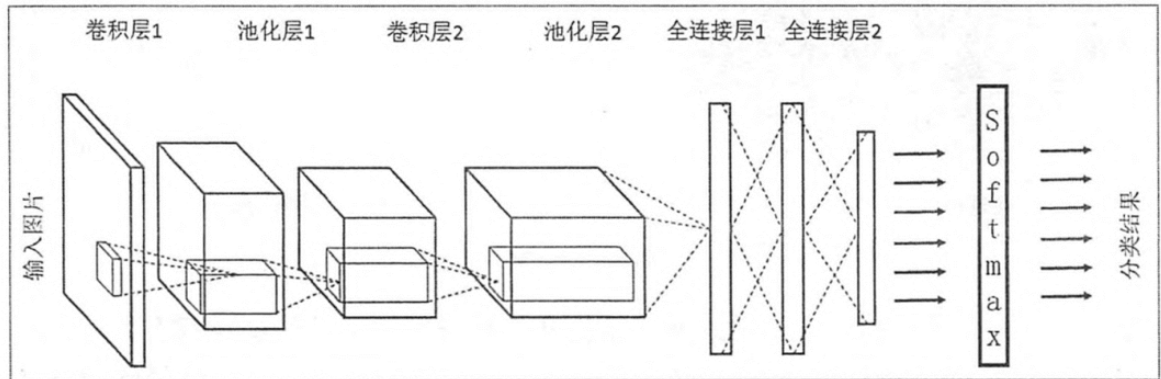
\includegraphics[width=1\textwidth]{CNN1}
  \caption{卷积神经网络结构示意图.}
  \label{fig_CNN1}
\end{figure}


深度神经网络提取特征的过程与其网络结构中的层有关。一般的步骤如下:

输入图片后,首先会对图片进行预处理以符合神经网络要求,随后在卷积层中会通过一组可学习的滤波器对输入图片进行滤波操作,提取出图像不同位置、方向以及大小的特征。通过多个滤波器对同一张图片进行卷积操作,就可以得到多个输出结果(即特征图)。同时,在卷积操作中还会加入偏置项,并使用激活函数增加非线性。

在池化层中通过对每个特征图区域内的像素值进行降维和采样,可以减少参数数量和计算量,并增强模型的鲁棒性。常见的池化操作有最大池化和平均池化。

全连接层将前面的卷积层和池化层的输出展平为一维向量,并通过多个全连接层进行分类或回归等任务。

Softmax层用于将全连接层的输出转换为概率分布。

基于深度学习的端到端方法(end-to-end)可以将原始数据直接输入网络,通过网络中多层非线性变换自动学习到数据中心最具有代表性和区分行的特征。

也有一种基于迁移学习的方法,利用已经训练好的深度神经网络在新任务上进行微调,来满足新任务的需求。这种方法可以大大减少训练时间和训练所需的样本数量,还能够提高模型泛化能力。常见的基于迁移学习的方法包括使用预训练模型进行微调、使用对抗生成网络进行特征生成等。

深度神经网络的特殊结构和参数化使其在当前的计算机视觉中取得了较大成功。当前在图像搜索领域存在AlexNet、VGG、GoogLeNet、ResNet和MobileNet等网络模型作为特征提取的基础\citep{CBIRSHORT}。

(1)AlexNet。AlexNet是2012年ImageNet的冠军模型,相比往年模型AlexNet极大的提高了检索结果准确率,让CNN成为了图像分类的核心算法模型。模型结构由5个卷积层和3个全连接层组成。还开创性地采用了双GPU并行技术,将卷积层分为两份分别计算,减轻GPU压力。为了防止网络过拟合而导致结果不佳,AlexNet使用Dropout将部分输出变为0。此外AlexNet还开创性地提出局部响应归一化(Local Response Normalization,LRN),使得模型的泛化能力更强。

(2)VGGNet。VGGNet拥有1×1的卷积核。更小的卷积核代替大的卷积核能增加网络的深度,可以减少参数量,实现不同通道间的融合。最后的全连接层变为1X1的卷积层,维数低便于检索计算。目前VGG16与VGG19使用较多,两者分别拥有13层和16层卷积层。

(3)GoogLeNet。GoogLeNet针对图像中突出部分的大小差异大的问题提出了多样卷积核。在每一层都用多个不同尺寸的卷积核去进行卷积操作。不仅解决了问题,并且减少了参数数量、增加了网络深度。现在使用较多的有inceptionV3和inceptionV4模型。

(4)ResNet。ResNet针对网络退化的问题提出了残差网络。由于之前网络都是逐层相连,一层一层往下输出的,因此只要其中一层学习特征失败,则之后的每一层都会失败,以至于输出结果不理想,导致网络深度难以加深。对此ResNet中提出的残差网络解决了此问题。ResNet在网络中加入了n条跳链,让网络中的每一层都不只能看到它前一层的输出值,还能看到更前层的输出。因此,如果它前一层学习失败,它便会将更前层的输出值作为自己的输入值,不再只受前一层的影响。

(5)MobileNet。相较于其他模型,MobileNet算是一个轻量级的神经网络,当设备性能受限、对准确率要求并不高或对效率要求较高时,MobileNet可以作为一个选择。

在图像检索的实际应用中,由于模型本身的固有特性,检索结果也会受到这样或那样的影响。开发者们通常也会对模型进行一些客制化(customization)。例如进行特征融合进行互补。Li\citep{Li}就在多层无序池的基础上提出多层无序融合(Multi-layer Orderless Fusion,MOF)算法,在UKBench(伦敦的椅子图像数据集,有10200张图片)数据集的实验证明,融合卷积层与全连接层(fully connected layers,FC)性能更优。还有学者认为模型间融合可弥合中级和高级特征之间的差距,例如结合VGG-19与AlexNet学习组合特征,可以互补两个模型的优点。

\section{研究内容}

本项目的研究目标是设计一个基于Python的图像搜索引擎。最终的结果是一个CBIR的图像搜索引擎。

1.阅读相关学术论文资料了解图像搜索引擎的结构和发展、国内外研究现状以及适合加入项目的模型或技术。

2.明确设计结构:用户交互界面,特征提取,图像预处理,相似度算法,数据库。

3.了解和使用可能会使用到的Python库文件。如tensorflow(深度学习平台)、numpy(存储和处理大型矩阵)、pillow(图像处理库)、flask(网络架构库)等等。

4.在预训练模型中选取合适的模型输出,编写对应的前端和后端程序,实现图像搜索功能。

5.选取合适的评估方法对引擎性能进行评估,如TOP-K等。

6.对程序进行功能扩展。探讨引擎的可能的应用场景,以及项目可持续发展的前景。


\chapter{程序总体设计}

\section{算法设计}

基于python的图像搜索引擎步骤基本都脱离不了图1-2中的CBIR一般框架,其算法总体设计可以包括以下几个步骤:

1. 图像测试数据库的准备:从网络获取图片数据集,并对图片进行预处理,如调整大小、裁剪等,以便后续处理。大多数模型对输入图像是有特定要求的,所以这步不可或缺。

2. 特征提取:使用深度学习模型(如卷积神经网络)对每张图片进行特征提取,将图片转化为向量表示。这里可以使用已经训练好的模型(如VGG、ResNet等),也可以自己训练、客制化模型。随后将提取后的向量存储在数据库中方便使用。

3. 特征对比:当用户在网页中输入一张图片时,使用同样的特征提取方法将其转化为向量表示,并在数据库中进行运算查找与之最相似的图片。这里可以使用欧氏距离、余弦相似度或汉明距离等方法计算相似度。

4. 结果展示:将检索到的相似度最高的图片返回给用户网站,并提供相关信息(如描述等)。

\begin{figure}[!htb]
  \centering
  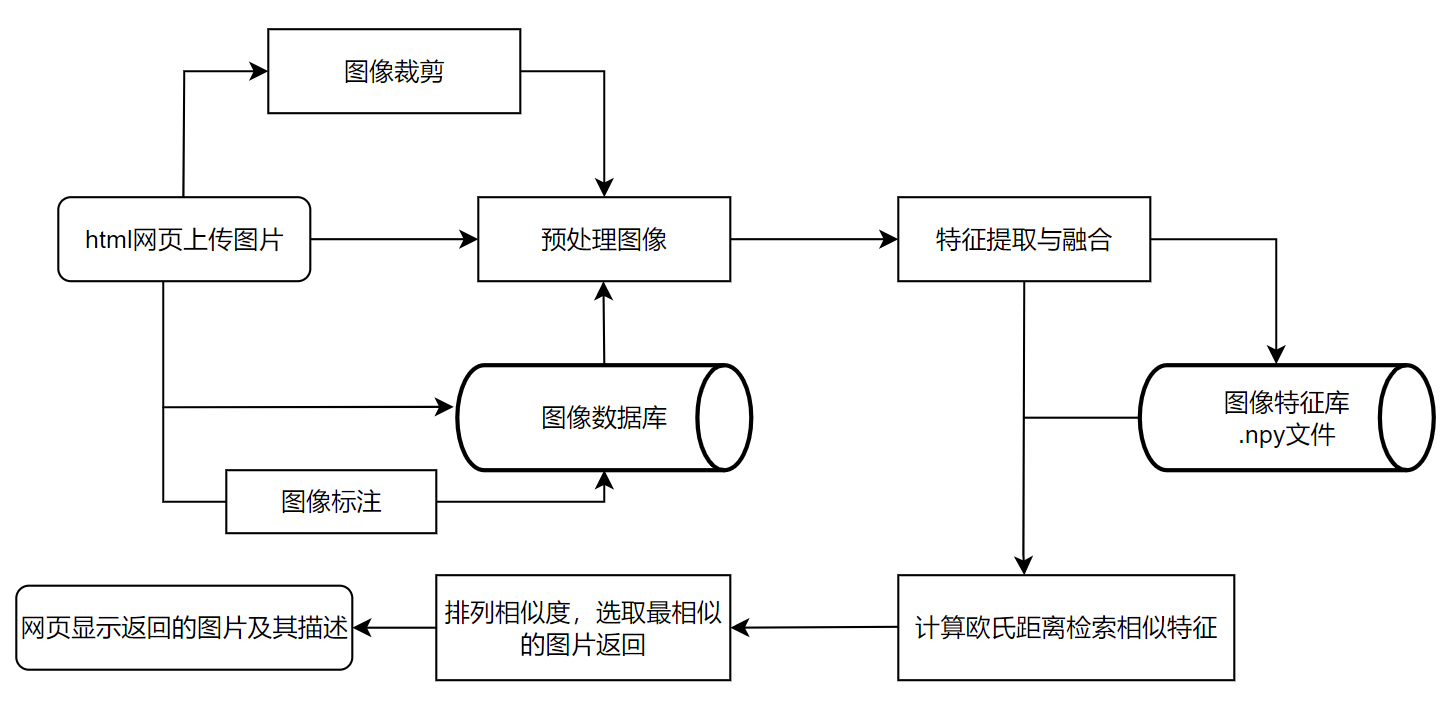
\includegraphics[width=1\textwidth]{totalimage}
  \caption{总体程序流程.}
  \label{fig_totalimage}
\end{figure}

\section{程序运行环境的搭建以及运行设备信息}

\subsection{程序运行环境搭建}

在运行设计一个新的、需要诸多库文件的Python项目的时候,由于不同项目为了实现特定的功能需要不同特定版本的库文件,而为了不让不同项目相互干扰,一般的建议是创建一个虚拟环境。虚拟环境可以隔绝项目之间依赖项和Python解释器版本,这样我们就可以在一台计算机上同时使用多个不同版本的Python库且不冲突。

python3 -m venv tensorflow

在命令行输入上述指令可以创建一个名为“tensorflow”的虚拟环境,随后便可以激活环境安装库文件了。本论文中我们都将使用“tensorflow”作为虚拟环境的名称。环境激活与退出命令分别如下:

activate tensorflow

conda.bat deactivate

在安装库文件前,还有一件事要做,由于本项目使用的是tensorflow-GPU(可以使用GPU加速,大大加快一些进程)版本,需要先去查询对应的稳定python、CUDA、cuDNN、编译器和构建工具的版本。例如本项目的python版本是3.19.3,对应的tensorflow-GPU版本是2.5.0,MSVC2019,BAZEL3.7.2,cuDNN8.1,CUDA11.2。其他具体信息可以前往tensorflow官网进行查询。

官网地址:https://tensorflow.google.cn/install/source$\_$windows?hl=zh-cn

下面是程序运行所需要的Python库文件及其版本号(若无标明版本号则表明最新版本即可,可以使用pip依次下次下列库文件):

tensorflow=2.5.0

Pillow

Flask

Flask-avatars

numpy=1.19.5

os

pathlib

base64

\subsection{设备信息}

笔记本电脑型号:Dell G3 3590

独立显卡型号:NVIDIA GeForce GTX 1660TI with Max-Q Design

中央处理器型号:Intel(R) Core(TM) i7-7950H @2.60HZ

内存型号:海力士16G 2666MHZ x 2

硬盘型号:英睿达MX500 SATA3.0 

\section{图像搜索引擎项目文件设计}

项目的图像搜索引擎主要分为数据库、特征提取函数、特征提取脚本、服务器脚本。流程参考图2-1。

\begin{figure}[!htb]
  \centering
  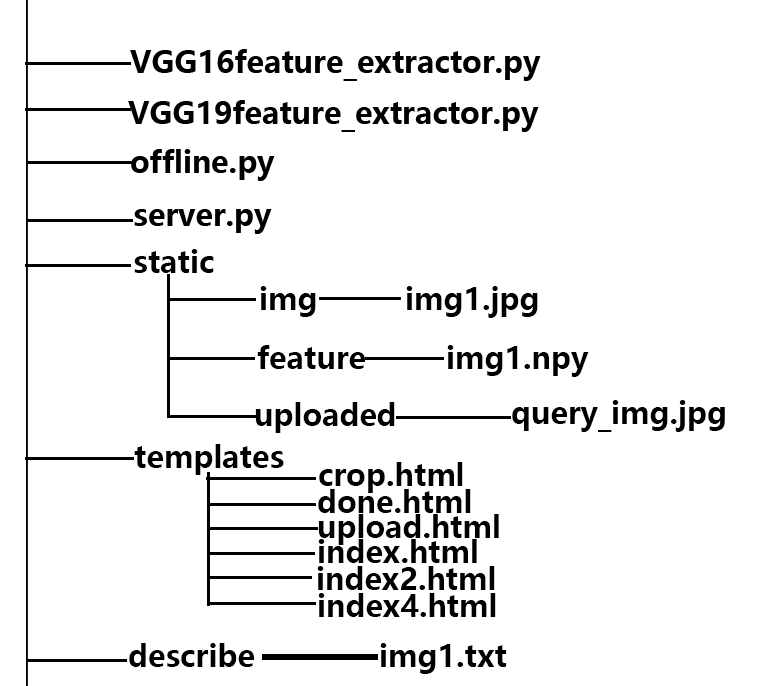
\includegraphics[width=0.75\textwidth]{structure}
  \caption{项目文件一览图.}
  \label{fig_structure}
\end{figure}

数据库包括static中的img、feature中分别存放的图片和图片特征文件,uploaded中则存放着用户上传的图片。describe中是图片对应的描述。

两个feature$\_$extractor对应着不同的模型特征提取方法,分别是VGG16的fc1和VGG19的fc2输出。

offline.py是特征提取脚本,利用上述的脚本将图片特征提取出来存储在同名特征文件中。

server.py是服务器脚本,用于开设网页提供用户交互界面和实现相似度计算功能并返回图片。

templates中是服务器返回的用户交互网页html文件。具体要实现的功能在下面代码中会说明。


\section{特征提取函数VGG16feature$\_$extractor.py设计}

设计程序需要先引入库文件,方便后续使用,为了保持代码简洁性引入库够用即可,特征提取函数需要引入库文件如下:

from tensorflow.keras.preprocessing import image

from tensorflow.keras.applications.vgg16 import VGG16, preprocess$\_$input

from tensorflow.keras.models import Model

import numpy as np

import os

在上述代码中引入tensorflow.keras的图像预处理功能,因为模型都有不同的输入数据要求,要根据具体模型而决定。例如VGG-16的输入必须是224x224像素的图片。在这里引入了keras自带的VGG16模型作为体系架构,同时还引入了numpy库对特征向量进行处理。

为了应对一些GPU不能使用的特殊情况,可以使用下面这段代码禁用GPU,只使用CPU:

os.environ["CUDA$\_$VISIBLE$\_$DEVICES"]="-1"

通常来说强烈建议使用GPU,尤其是当数据库较大的时候,CPU的处理图像的速度过慢,使用GPU加速可以节省大量时间,加强引擎响应性能。

下面是代码正文:

class VGG16FeatureExtractor:

\qquad def $\_$$\_$init$\_$$\_$(self):

\qquad \qquad base$\_$model = VGG16(weights='imagenet')

\qquad \qquad self.model = model(inputs=base$\_$model.input, outputs=base$\_$model.get$\_$

\qquad \qquad layer('fc1').output)

\qquad def extract(self, img):

\qquad \qquad img = img.resize((224, 224))

\qquad \qquad img = img.convert('RGB')

\qquad \qquad x = image.img$\_$to$\_$array(img)

\qquad \qquad x = np.expand$\_$dims(x, axis=0)

\qquad \qquad x = preprocess$\_$input(x)

\qquad \qquad feature = self.model.predict(x)[0]

\qquad \qquad return feature / np.linalg.norm(feature)

在上述的代码中,程序载入了VGG16模型作为基本架构,并使用了imagenet预先训练的权重,随后在网络中选择了fc1层(全连接层)作为输出,也就是说最终输出的是图像的全局特征。至于选择哪一层、反映的什么特征并无硬性要求,可以根据图像检索引擎的具体需求来决定。

由于VGG16网络对于输入图像的要求,先用resize函数将输入函数大小重塑为224x224像素的图片。并确保图像是RGB模式的。随后用将图片转为图片数量(1)、长、宽、通道的数组,再用先前引入的preprocess$\_$input函数减去每个像素的平均值预测得到fc1层的输出,返回该输出特征值。

VGG19feature$\_$extractor.py代码与上述内容内容基本一致,将所有的VGG16替换为VGG19即可。

\section {特征提取脚本offline.py设计}

特征提取脚本的作用是预先将数据库中的图像特征提取并储存起来,保存在与图片同名的.npy文件中,便于后续进行使用。下面是offline.py的代码:

from PIL import Image

from VGG16feature$\_$extractor import VGG16FeatureExtractor

from VGG19feature$\_$extractor import VGG19FeatureExtractor

from pathlib import Path

import numpy as np

if $\_$$\_$name$\_$$\_$ == '$\_$$\_$main$\_$$\_$':

\qquad VGG19fe = VGG19FeatureExtractor()

\qquad VGG16fe = VGG16FeatureExtractor()
    
\qquad for img$\_$path in sorted(Path("./static/img").glob("*.jpg")):

\qquad \qquad print(img$\_$path)

\qquad \qquad feature = VGG16fe.extract(img=Image.open(img$\_$path))

\qquad \qquad VGG16feature$\_$path = Path("./static/VGG16feature") / (img$\_$path.stem + ".npy") 

\qquad \qquad np.save(VGG16feature$\_$path, feature)

\qquad \qquad feature = VGG19fe.extract(img=Image.open(img$\_$path))

\qquad \qquad VGG19feature$\_$path = Path("./static/VGG19feature") / (img$\_$path.stem + ".npy")  

\qquad \qquad np.save(VGG19feature$\_$path, feature)

这里我们引用了两个特征提取函数,便于后面研究不同模型不同输出层的效果。还用了pathlib用于存储路径。用 for xx in sorted遍历/static/img文件夹中的图片,分别用两个提取函数提取特征存储于模型对应的.npy文件中。如果没有新图片的加入无需再次运行。

\section {网络模块server.py与index.html设计}

flask是一个轻量级的网络架构,适合快速搭建功能简单的网站。flask很方便的一点在于可以创建不同的url来创建多个网页实现更多功能,可以保持代码的简洁性。

$\#$server.py的图像搜索功能代码

import numpy as np

from VGG16feature$\_$extractor import VGG16FeatureExtractor

from VGG19feature$\_$extractor import VGG19FeatureExtractor

from datetime import datetime

from PIL import Image, ImageDraw, ImageFont

from flask import Flask,render$\_$template,request

from pathlib import Path

import base64

app=Flask($\_$$\_$name$\_$$\_$)

VGG16fe = VGG16FeatureExtractor()

VGG19fe = VGG19FeatureExtractor()

VGG16features = []

VGG19features = []

VGG16img$\_$paths = []

VGG19img$\_$paths = []

\qquad \qquad $\#$将数据库中的jpg文件及其npy文件一一对应

for VGG16feature$\_$path in Path("./static/VGG16feature").glob("*.npy"):

\qquad VGG16features.append(np.load(VGG16feature$\_$path, encoding='bytes',

\qquad allow$\_$pickle=True))

\qquad VGG16img$\_$paths.append(Path("./static/img") / (VGG16feature$\_$

\qquad path.stem + ".jpg"))

VGG16features = np.array(VGG16features)

for VGG19feature$\_$path in Path("./static/VGG19feature").glob("*.npy"):

\qquad VGG19features.append(np.load(VGG19feature$\_$path, encoding='bytes', 

\qquad allow$\_$pickle=True))

\qquad VGG19img$\_$paths.append(Path("./static/img") / (VGG19feature$\_$

\qquad path.stem + ".jpg"))

VGG19features = np.array(VGG19features)

@app.route('/VGG16', methods=['GET', 'POST'])

def\quad VGG16():

\qquad if request.method == 'POST':

\qquad \qquad file = request.files['query$\_$img']

\qquad \qquad $\#$ 获取网页端上传的图片并保存

\qquad \qquad img = Image.open(file.stream)  $\#$ PIL image

\qquad \qquad uploaded$\_$img$\_$path = "static/uploaded/" + "VGG16"

\qquad \qquad + datetime.now().isoformat().replace(":", ".") + "$\_$"

\qquad \qquad + file.filename

\qquad \qquad img.save(uploaded$\_$img$\_$path)

\qquad \qquad $\#$ 提取特征,与数据库特征进行比对,用欧式距离计算图片相似度

\qquad \qquad query = VGG16fe.extract(img)

\qquad \qquad dists = np.linalg.norm(VGG16features-query, axis=1)  

\qquad \qquad ids = np.argsort(dists)[:30]

\qquad \qquad $\#$对计算结果进行排序,选取相似度最高的三十张图片返回

\qquad \qquad scores = [(dists[id], VGG16img$\_$paths[id]) for id in ids]
        
\qquad \qquad desc=scores[0]

\qquad \qquad textdesc=''.join(str(i) for i in desc)

\qquad \qquad textdesc2=textdesc.split(' \textbackslash  \textbackslash ')[2].rsplit('$\_$', 2)[-3]

\qquad \qquad $\#$选取相似度最高的图片在describe文件夹中寻找描述文件返回

\qquad \qquad with open("describe/"+textdesc2 + ".txt","r", encoding='utf-8') as file:

\qquad \qquad \qquad describe=file.read()
        
\qquad \qquad VGG16describe="你正在使用VGG16模型"

\qquad \qquad $\#$ 用render$\_$template对网页端进行渲染,返回图像、文本描述等
        
\qquad \qquad return render$\_$template('index.html', model$\_$describe=VGG16describe

\qquad \qquad ,query$\_$describe=describe,query$\_$path=uploaded$\_$img$\_$path,

\qquad \qquad scores=scores)

\qquad else:

\qquad \qquad return render$\_$template('index.html')

@app.route('/VGG19', methods=['GET', 'POST'])

def\quad VGG19():

\qquad .....

\qquad $\#$urlVGG19的代码与urlVGG16的代码基本一致,全部替换即可


if $\_$$\_$name$\_$$\_$=="$\_$$\_$main$\_$$\_$":

\qquad app.run("0.0.0.0", debug=True)

\qquad $\#$运行服务器,在浏览器输入localhost:5000/VGG16使用,可以使用网页按钮切换模型

$\#$index.html


<!doctype html>

<html>

<body>

<a href = "crop">

<button>预处理图像</button>

</a>

<a href = "label1">

<button>标注图片</button>

$\#$下方是五个在不同url之间切换的按钮

</a>

<a href = "upload">

<button>上传图片至数据库</button>

</a>

<a href = "VGG19">

<button>切换至VGG19模型</button>

</a>

<a href = "VGG16">

<button>切换至VGG16模型</button>

</a>

<div class="container">

<h1>基于Python的简易图像搜索引擎</h1>

$\#$提交图片

<form method="POST" enctype="multipart/form-data">

<input type="file" name="query$\_$img"><br>

<input type="submit">

</form>

<h2>搜索图像:</h2>

$\#$上传的图片会展示在这里

$\{$ $\%$ if query$\_$path $\%$$\}$

<img src="{{ query$\_$path }}" width="300px">

$\{$ $\%$ endif $\%$ $\}$

$\#$这里是对模型的描述

<div id="model$\_$describe">{{model$\_$describe}}<div>

$\#$这里是根据结果所返回的一个可能的图片描述

<h2>你可能在找:<h2>

<div id="query$\_$describe">{{query$\_$describe}}<div>

$\#$展示搜索结果图片和相似度,可以在server.py里调整返回图片数量和相似度

<h2>搜索结果:</h2>

$\{$ $\%$ for score in scores $\%$ $\}$

<figure style="float: left; margin-right: 20px; margin-bottom: 20px;">

<img src="{{ score[1] }}" height="200px">

<figcaption>{{ score[0] }}</figcaption>

</figure>

$\{$ $\%$ endfor $\%$ $\}$

</div>

</body>

</html>

\section {扩展功能}

实现基础的图像搜索后,还研究实现整合了一些与图像相关的扩展功能。这些扩展功能的实现都是通过在flask框架内添加url来实现的。所需的库文件在上述server.py已经全部导入,所以下面不会再次引入。

\subsection {基于flask-avatars的仿labelme标注功能}

近年的多数的图像研究都会涉及到图像标注方面。而labelme作为一个功能齐全的标注平台传播与使用也较为广泛,但由于labelme官网近期已经停止发放注册账号,所以制作一个网页版仿labelme的扩展功能是有一定实践意义的。

\begin{figure}[!htb]
  \centering
  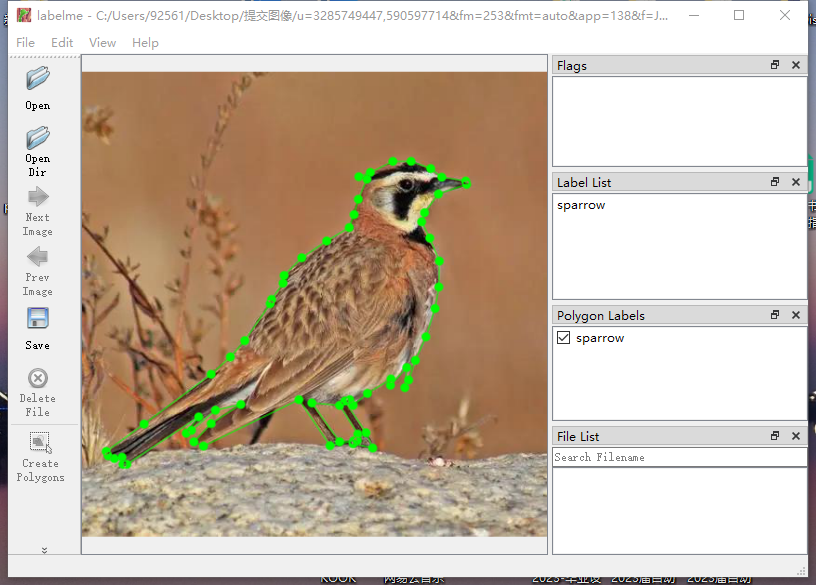
\includegraphics[width=0.8\textwidth]{labelme}
  \caption{labelme实例,标注了麻雀的轮廓和名称.}
  \label{fig_labelme}
\end{figure}

\begin{figure}[!htb]
  \centering
  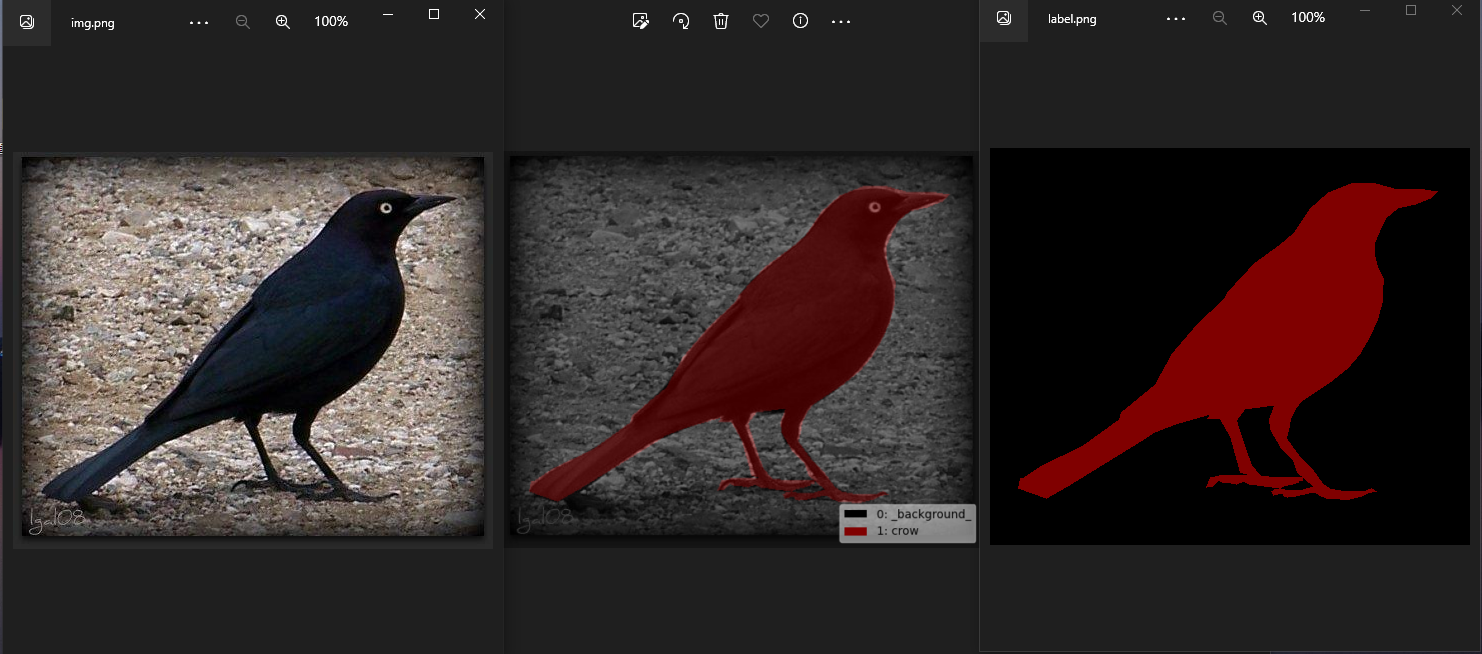
\includegraphics[width=0.8\textwidth]{labelme2}
  \caption{labelme实例,利用labelme自带脚本处理后的返回图像.}
  \label{fig_labelme2}
\end{figure}



flask-avatars原先是一个用于生成头像的库,集成了jcrop等功能。在实现的程序中,我们可以通过网页上传图像,框选想要标注的范围,后端会获得框选坐标信息,用pillow库对图像进行处理并返回到网页中。项目中根据给出的实例(原代码地址https://blog.csdn.net/szyyzt/article/details/102463174)头像生成代码进行了改进,实现了标注功能。总共分为三步,用户上传图像,用户框选标注范围,返回给用户标注过的图像,图像结果是类似于labelme的。下面给出范例和实现代码:

\begin{figure}[!htb]
  \centering
  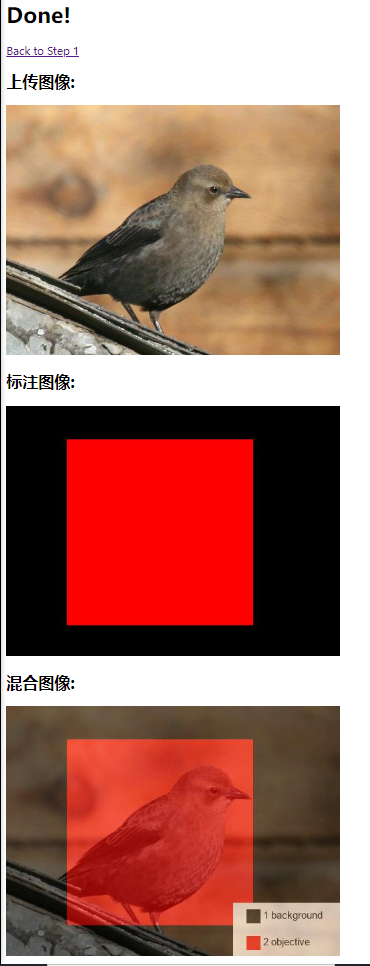
\includegraphics[width=0.50\textwidth]{label}
  \caption{标注结果演示.}
  \label{fig_label}
\end{figure}

$\#$关于标注功能的上传文件放在项目新建文件夹labeled中。

$\#$app.secretkey可随便设置一个

app.secret$\_$key='19062314'

$\#$这里是设置上传文件的存储位置,设定为项目中的labeled文件夹

app.config['AVATARS$\_$SAVE$\_$PATH']='labeled/'

@app.route('/avatars/<path:filename>')

def get$\_$avatar(filename):

\qquad return send$\_$from$\_$directory(app.config['AVATARS$\_$SAVE$\_$PATH'], filename)

@app.route('/label1', methods=['GET', 'POST'])

def label1():

$\#$获取网页端上传的文件,一份存储在进程session中用于网站选框,一份存储在labeled文件夹中

\qquad if request.method == 'POST':

\qquad \qquad file1 = file2 = request.files.get('file')

\qquad \qquad raw$\_$filename = avatars.save$\_$avatar(file1)

\qquad \qquad session['raw$\_$filename'] = raw$\_$filename
   
\qquad \qquad upload$\_$path=("./labeled/uploaded.jpg")

\qquad \qquad img=Image.open(file2)

\qquad \qquad img.save(upload$\_$path)

$\#$获取文件完毕后,网页端url跳转至label2中

\qquad \qquad return redirect(url$\_$for('label2'))

\qquad return render$\_$template('upload.html')
    
@app.route('/label2', methods=['GET', 'POST'])

def label2():

\qquad if request.method == 'POST':

$\#$获取用户的选框信息

\qquad \qquad x = request.form.get('x')

\qquad \qquad y = request.form.get('y')

\qquad \qquad w = request.form.get('w')

\qquad \qquad h = request.form.get('h')
            
$\#$由于获得信息的是字符串,无法直接使用,我们这里先将用户的选框信息转为浮点数便于使用

\qquad \qquad x1=float(x)

\qquad \qquad y1=float(y)

\qquad \qquad w1=float(w)

\qquad \qquad h1=float(h)
            
$\#$打开上传的图片,用size获取图片的大小

\qquad \qquad img=Image.open("./labeled/uploaded.jpg")

\qquad \qquad width, height = img.size
            
$\#$用pillow库生成与原图像大小一致的图像,在上面用选框信息进行一系列标注处理

\qquad \qquad pic3 = pic1 = Image.new('RGB', (width,height), 'black')
            
\qquad \qquad draw = ImageDraw.Draw(pic1)

\qquad \qquad draw.rectangle((x1, y1, x1+w1, y1+h1), outline="red", fill='red')

\qquad \qquad pic1.save('./labeled/background.jpg')
            
\qquad \qquad draw1 = ImageDraw.Draw(pic3)

\qquad \qquad draw1.rectangle((x1, y1, x1+w1, y1+h1), outline="red", fill='red')

\qquad \qquad draw1.rectangle(( width-160 , height-80, width , height ),fill='white')

\qquad \qquad draw1.rectangle(( width-140 , height-70 , width-120 , height-50 ), 

\qquad \qquad fill='black')

\qquad \qquad draw1.rectangle(( width-140 , height-30 , width-120 , height-10 ), 

\qquad \qquad fill='red')

            
\qquad \qquad font=ImageFont.truetype('arial.ttf',15)

\qquad \qquad text$\_$color=(0,0,0)

\qquad \qquad draw1.text((width-115,height-70),'1 background', font=font, 

\qquad \qquad fill=text$\_$color)

\qquad \qquad draw1.text((width-115,height-30),'2 objective', font=font, fill=text$\_$color)

            
\qquad \qquad pic2=Image.open('./labeled/uploaded.jpg')

$\#$混合图像,使结果更直观

\qquad \qquad miximg=Image.blend(pic3, pic2, 0.45)

\qquad \qquad miximg.save('./labeled/miximg.jpg')

$\#$分别将上传图像、标注图像、混合图像编码为base64字符串,方便显示

\qquad \qquad with open('./labeled/uploaded.jpg','rb') as img$\_$file:

\qquad \qquad \qquad data1 = img$\_$file.read()

\qquad \qquad \qquad imgdata1 = base64.b64encode(data1).decode("utf-8")
                
\qquad \qquad with open('./labeled/background.jpg','rb') as img$\_$file:

\qquad \qquad \qquad data2 = img$\_$file.read()

\qquad \qquad \qquad imgdata2 = base64.b64encode(data2).decode("utf-8")
                
\qquad \qquad with open('./labeled/miximg.jpg','rb') as img$\_$file:

\qquad \qquad \qquad data3 = img$\_$file.read()

\qquad \qquad \qquad imgdata3 = base64.b64encode(data3).decode("utf-8")
                
$\#$使用render$\_$template 渲染用户网页返回图像

\qquad \qquad return render$\_$template('done.html', img$\_$data1=imgdata1, 

\qquad \qquad img$\_$data2=imgdata2, img$\_$data3=imgdata3 )

\qquad return render$\_$template('crop.html')

$\#$图片上传网站upload.html

<!DOCTYPE html>

<html lang="en">

<head>

<meta charset="UTF-8">

<title>Flask-Avatars</title>

</head>

<body>

<h1>Step 1: Upload</h1>

$\#$用户上传图片

<form method="post" enctype="multipart/form-data">

<input type="file" name="file">

<input type="submit">

</form>

</body>

</html>

$\#$选框标注网站crop.html

<!DOCTYPE html>

<html lang="en">

<head>

<meta charset="UTF-8">

<title>Flask-Avatars</title>

{{ avatars.jcrop$\_$css() }}

<style>

$\#$preview-box {

display: block;

position: absolute;

top: 10px;

right: -280px;

padding: 6px;

border: 1px rgba(0, 0, 0, .4) solid;

background-color: white;

-webkit-border-radius: 6px;

-moz-border-radius: 6px;

border-radius: 6px;

-webkit-box-shadow: 1px 1px 5px 2px rgba(0, 0, 0, 0.2);

-moz-box-shadow: 1px 1px 5px 2px rgba(0, 0, 0, 0.2);

box-shadow: 1px 1px 5px 2px rgba(0, 0, 0, 0.2);

}

</style>

</head>

<body>

<h1>Step 2: Crop</h1>

{{ avatars.crop$\_$box('get$\_$avatar', session['raw$\_$filename']) }}

{{ avatars.preview$\_$box('get$\_$avatar', session['raw$\_$filename']) }}

<form method="post">

<input type="hidden" id="x" name="x">

<input type="hidden" id="y" name="y">

<input type="hidden" id="w" name="w">

<input type="hidden" id="h" name="h">

<input type="submit" value="Crop!">

</form>

{{ avatars.jcrop$\_$js() }}

{{ avatars.init$\_$jcrop() }}

</body>

</html>

$\#$标注图像展示网站done.html

<!DOCTYPE html>

<html lang="en">

<head>

<meta charset="UTF-8">

<title>Flask-Avatars</title>

</head>

<body>

<h1>Done!</h1>

<p><a href="/label1">Back to Step 1</a></p>

<h2>上传图像:</h2>

<img src="data:image/jpg;base64,{{img$\_$data1}}">

<h2>标注图像:</h2>

<img src="data:image/jpg;base64,{{img$\_$data2}}">

<h2>混合图像:</h2>

<img src="data:image/jpg;base64,{{img$\_$data3}}">

</body>

</html>

\subsection {图像裁剪预处理功能}

全局特征和局部特征各有优劣之处。当图片中有多个目标特征时可能会污染特征提取,干扰后续相似度计算,以至于最终不能返回用户所需要的的图片。那么如果用户可以对上传图像进行裁剪预处理就可以更灵活地应对大多数情况。

\begin{figure}[!htb]
  \centering
  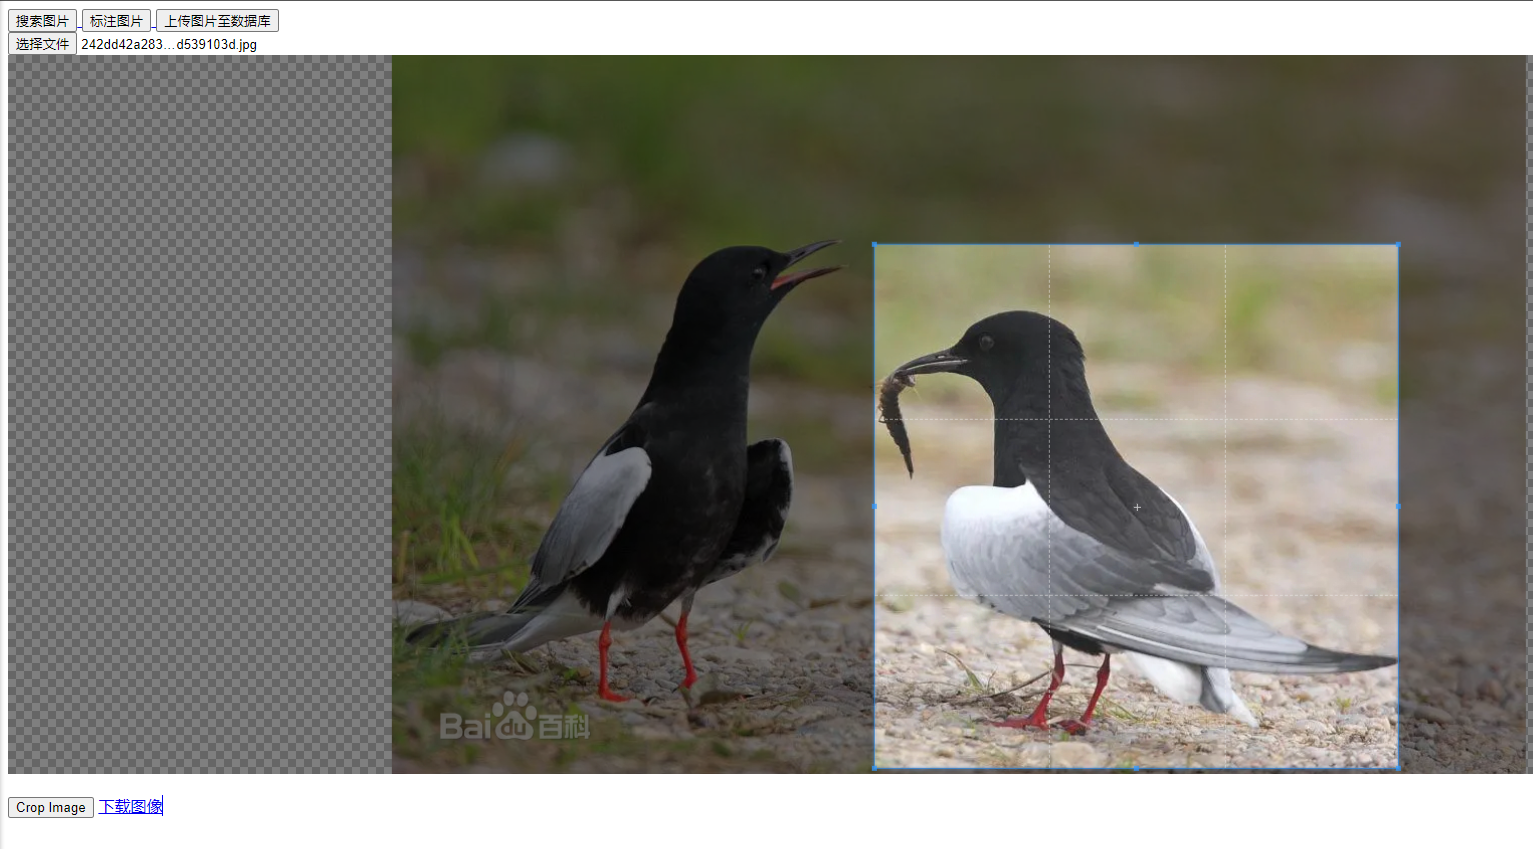
\includegraphics[width=1\textwidth]{crop1}
  \caption{裁剪功能演示,该图有两个目标,直接上传可能导致检索效果不好.}
  \label{fig_crop1}
\end{figure}

这里我们借用jquery和cropper插件的实例来完成,处理后的图片是一个224x224像素的图片,可以直接输入进模型。主要思路是上传图片,创建一个画布(canvas)来展示图片和框选想要裁剪图片的范围,点击按钮确定后创建一个新的224x224的画布,用于展示裁剪后的图片,点击下载按钮即可下载该图片。

\begin{figure}[!htb]
  \centering
  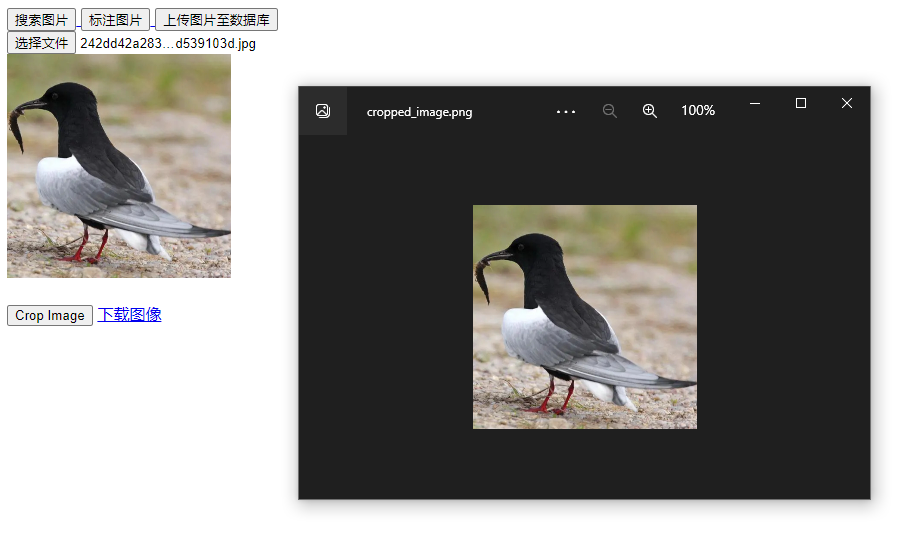
\includegraphics[width=1\textwidth]{crop2}
  \caption{裁剪功能演示,点击crop按钮裁剪后,点击下载按钮后下载的的图像.}
  \label{fig_crop2}
\end{figure}

$\#$python flask部分

@app.route('/crop', methods=['GET', 'POST'])

def crop():

\qquad return render$\_$template('index2.html')

$\#$index2.html

<!DOCTYPE html>

<html>

<head>

<title>图像裁剪预处理</title>

$\#$引入js插件脚本

<script src="https://cdnjs.cloudflare.com/ajax/libs/jquery/3.3.1/jquery.min.js">

</script>

<script src="https://cdnjs.cloudflare.com/ajax/libs/cropperjs/1.5.11/cropper.min

.js">

</script>

<link rel="stylesheet" href="https://cdnjs.cloudflare.com/ajax/libs/cropperjs/1.5.11/

cropper.min.css" />

</head>

<body>

<a href = "VGG16">

<button>搜索图片</button>

</a>

<a href = "label1">

<button>标注图片</button>

</a>

<a href = "upload">

<button>上传图片至数据库</button>

<br>

</a>

<input type="file" id="inputImage" name="file" accept="image/*">

<br>

<div>

<img id="image" src="" alt="Picture">

</div>

<br>

<div>

<button id="crop">Crop Image</button>

<a id="download" href="$\#$" download="cropped$\_$image.png">下载图像</a>

</div>

<script>

var cropper;

var image = document.getElementById('image');

var inputImage = document.getElementById('inputImage');

var crop = document.getElementById('crop');

var download = document.getElementById('download');

inputImage.addEventListener('change', function(e) {

var files = e.target.files;

var done = function(url) {

image.src = url;

cropper = new Cropper(image, {

aspectRatio: 1,

viewMode: 1,

preview: '.preview'

});

};

var reader;

var file;

var url;

if (files $\&$$\&$ files.length > 0) {
				
file = files[0];
				
if (URL) {
					
done(URL.createObjectURL(file));
				
} else if (FileReader) {
					
reader = new FileReader();
					
reader.onload = function(e) {
						
done(reader.result);
					
};
					
reader.readAsDataURL(file);
				
}
			
}
		
});

crop.addEventListener('click', function() {
			
var initialAvatarURL;
			
var canvas;
			
canvas = cropper.getCroppedCanvas({
				
width: 224,
				
height: 224,
			
});
			
initialAvatarURL = image.src;
			
image.src = canvas.toDataURL();
			
download.href = canvas.toDataURL();
			
cropper.destroy();
			
cropper = null;
		
});
	
</script>

</body>

</html>

\subsection {前端上传图像至后端数据功能}

这个模块的本质还是上传、存储文件,并且提取特征存储到相应文件中,只是指定的相对位置不同,加上使用OS库修改文件名后缀,这里不多做赘述。

\begin{figure}[!htb]
  \centering
  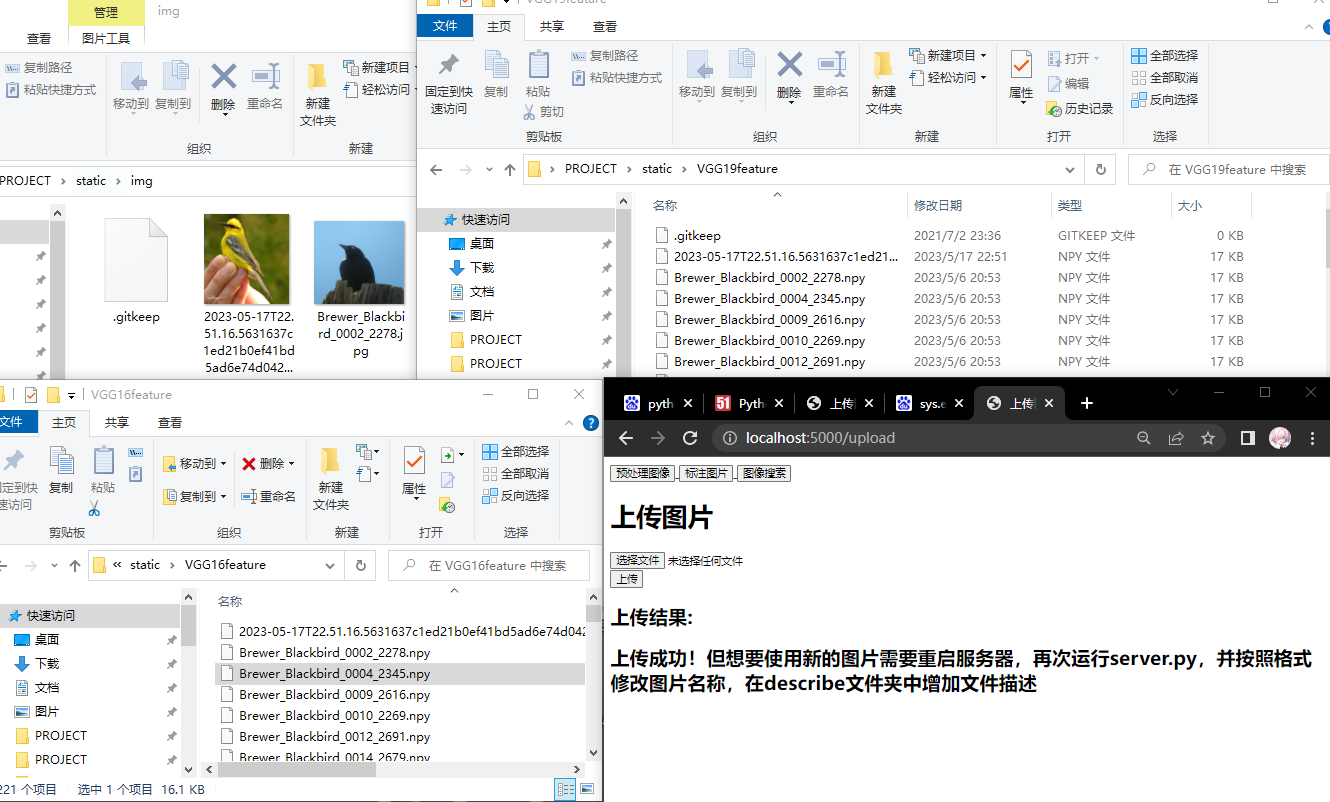
\includegraphics[width=1\textwidth]{upload}
  \caption{上传功能示例.}
  \label{fig_upload}
\end{figure}

如图所示,图片上传到数据库中后还进行了特征提取,无需再次运行offline.py花费大量时间,只需要重启服务器、修改文件名、增加文件描述即可使用新增的数据。

@app.route('/upload', methods=['GET', 'POST'])

def database():

\qquad if request.method == 'POST':

\qquad \qquad file = request.files['addtodatabaseimg']

\qquad \qquad img = Image.open(file.stream)

\qquad \qquad uploaded$\_$database$\_$img = datetime.now().isoformat().replace(":", ".") + 

\qquad \qquad file.filename
        
$\#$以两种方法提取图像特征

\qquad \qquad feature1 = VGG16fe.extract(img)

\qquad \qquad feature2 = VGG19fe.extract(img)
        
\qquad \qquad img.save("static/img/"+uploaded$\_$database$\_$img)

\qquad \qquad img.save("static/VGG16feature/"+uploaded$\_$database$\_$img)

\qquad \qquad img.save("static/VGG19feature/"+uploaded$\_$database$\_$img)
        
\qquad \qquad old$\_$form=".jpg"
        
\qquad \qquad dir$\_$path="static/VGG16feature/"

$\#$将制定文件夹中.jpg格式的文件转为.npy格式

\qquad \qquad for filename in os.listdir(dir$\_$path):

\qquad \qquad \qquad if filename.endswith(old$\_$form):

\qquad \qquad \qquad \qquad new$\_$filename1 = filename[:-len(old$\_$form)] + ".npy"

\qquad \qquad \qquad \qquad os.rename(os.path.join(dir$\_$path, filename), os.path.join(
  
\qquad \qquad \qquad \qquad dir$\_$path, new$\_$filename1))   
        
\qquad \qquad dir$\_$path="static/VGG19feature/"
        
\qquad \qquad for filename in os.listdir("static/VGG19feature/"):

\qquad \qquad \qquad if filename.endswith(old$\_$form):

\qquad \qquad \qquad \qquad new$\_$filename2 = filename[:-len(old$\_$form)] + ".npy"

\qquad \qquad \qquad \qquad os.rename(os.path.join(dir$\_$path, filename), os.path.join(
  
\qquad \qquad \qquad \qquad dir$\_$path, new$\_$filename2))   
        
$\#$将图像特征存在指定位置.npy文件中

\qquad \qquad np.save("static/VGG16feature/"+new$\_$filename1,feature1)

\qquad \qquad np.save("static/VGG19feature/"+new$\_$filename2,feature2)
        
\qquad \qquad uploadsuccess="上传成功!但想要使用新的图片需要重启服务器,再次运行server.py,并按照格式修改图片名称,在describe文件夹中增加文件描述"
        
\qquad \qquad return render$\_$template('index4.html',query$\_$describe=uploadsuccess)

\qquad else:

\qquad \qquad return render$\_$template('index4.html')



\chapter{图像搜索引擎性能测试以及分析}

\section{图像搜索引擎性能测试数据集介绍}

本项目用于测试引擎性能的数据集是加利福尼亚理工学院鸟类数据库(Caltech-UCSD Birds-200,CUB-200)。这个数据库有200种鸟类,共有11788张图片。每种约有50张。其中每个图像都标注有鸟的类别、边界框和关键点信息。这个数据集经常用语评估计算机视觉算法的性能。

\section{图像搜索引擎性能评价指标}

目前基于内容的图像检索主要有四种评价指标。分别是查准率(Precision)、查全率(又称召回率,Recall)、F-Score(混合了前两种度量,可调节两者权重)和均值平均精度(mAP)。

\subsection{查准率;准确率Precision}

查准率表示所有正确的检索图像占检索返回图像总数的比例。
\begin{equation}
  P = \frac{T}{T+U};
\end{equation}
其中T表示返回的相关图片的数量,其中U表示返回与不相关图片数量。

\subsection{召回率;查全率Recall}

召回率表示正确的检索图像占数据集相关的样本数量。
\begin{equation}
  R = \frac{T}{T+V};
\end{equation}
V表示数据集中未返回的与检索图像相关的样本数量。

\subsection{F-score}

F-Score表示召回率与精确率的加权调和平均值。
\begin{equation}
  R = \frac{(1+\beta^2)PR}{\beta^2(P+R)};
\end{equation}
调节β值可以控制Precision和Recall的权重。β<1,Precision更重要;β>1,Recall更重要;β=1,称为F1。

\subsection{均值平均精度mAP}

均值平均精度(mAP)是目前图像检索任务中最流行的评价指标。当给定一个查询q和top-K检索到数据的情况下,平均精度(AP)计算公式如下:
\begin{equation}
  AP(q) = \frac{1}{N}P(k)\alpha(k);
\end{equation}
其中k表示建所返回的第k个数据,P(k)表示返回前K个数据的精确度,N表示数据库中与当前查询图像q相关的图片数量。若第k个检索返回的数据与查询q相关,则α(k)=1,否则等于0。

mAP则是所有AP的平均值,计算公式如下:
\begin{equation}
  mAP = \frac{1}{Q}AP(q);
\end{equation}
Q代表查询样本总数。相较于其他性能评价指标,均值平均精度mAP更能反映全局性能。

在神经网络的性能衡量中,有一种更简易便捷同时可靠的的衡量方法——top-k accuracy,即前k张图片中是否有与搜索图相关的图片。一般情况下是选取TOP-1和TOP-5的准确率。

\section{图像搜索引擎检索结果分析}

从数据库内随机选取某种鸟类图片进行测试。
\begin{figure}[!htb]
  \centering
  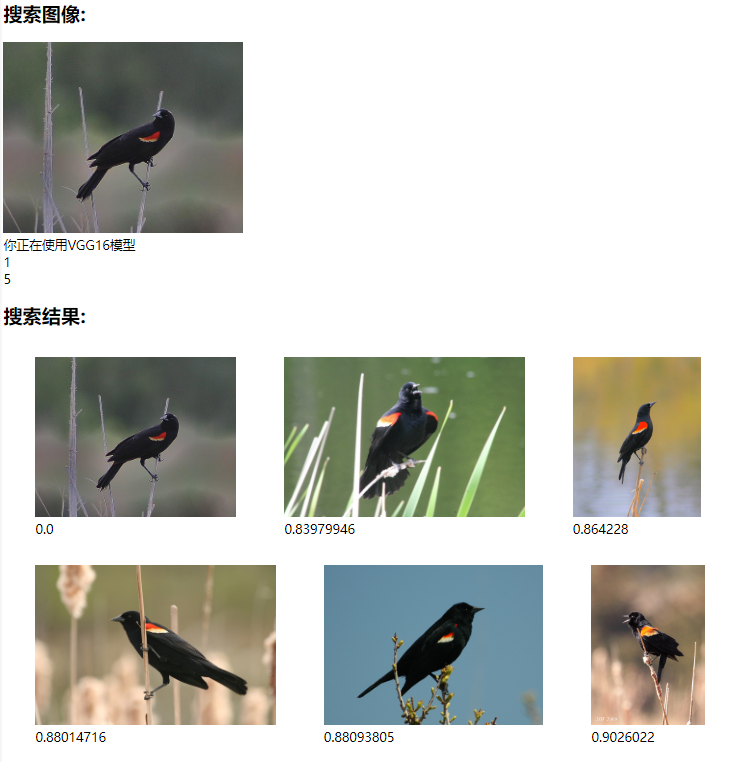
\includegraphics[width=0.45\textwidth]{result1}
  \caption{搜索结果示例图.}
  \label{fig_result1}
\end{figure}

如图3-1,返回的第一张图片就是上传的图片,不用作结果计算。由于精度(P)、召回率(R)具体结果受返回图像数量影响较大,在此不用做评价指标。这里我们使用在神经网络性能指标中常用的top-K 精度。若第二张图片相关,则top-1精确度是100$\%$。若第二到第六有相关图片,则top-5精确度为100$\%$,否则都为0。最终结果取平均值。各模型输出分别进行100次测试,下面给出TOP-K准确率结果数据表格:

\begin{table}[h]
  \caption{检索结果表格}
\centering
\setlength{\tabcolsep}{5mm}{
\begin{tabular}{|c|c|c|c|}
\hline
模型输出  & Top-1准确率 &  Top-5准确率      &   前五张总准确率     \\ \hline
VGG16fc1  & 79.0$\%$    &   87$\%$         &   68.2$\%$      \\ \hline
VGG19fc2  & 80.0$\%$    &   90$\%$         &   65.0$\%$      \\ \hline
\end{tabular}}
\label{gra_process}
\end{table}

从结果我们可以看出两个模型输出的top-K准确率准确率相近,TOP1都在80$\%$左右,TOP-5在90$\%$左右,前五张准确率在67$\%$左右。网页响应速度也较快,约0.1秒。一般来说,使用CUB-200作为测试数据集时,较好的模型top-1在70$\%$以上,top-5在90$\%$以上。这也说明该程序算法的性能还是较为理想的。

\begin{figure}[!htb]
  \centering
  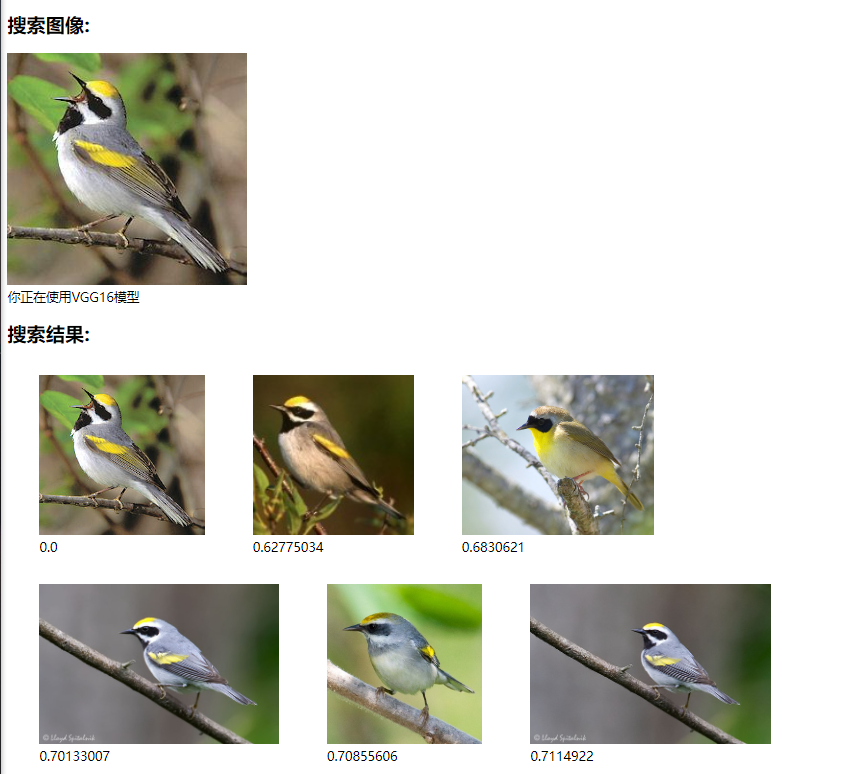
\includegraphics[width=0.75\textwidth]{PIC5}
  \caption{高对比度饱和度色差鸟类.}
  \label{fig_PIC5}
\end{figure}

对具体的检索结果个体进行分析,如图3-2可以注意到模型对颜色更鲜艳的鸟类,也就是图片局部拥有更高色差、饱和度的图片识别结果更准确,如黄色、橙色、红色、鲜蓝色等等。这些颜色在自然界中的出现较少,用于图像识别检索效果较为理想。

另外还能得到模型对有一定规则纹理的鸟类识别结果更为准确,如图3-3。

\begin{figure}[!htb]
  \centering
  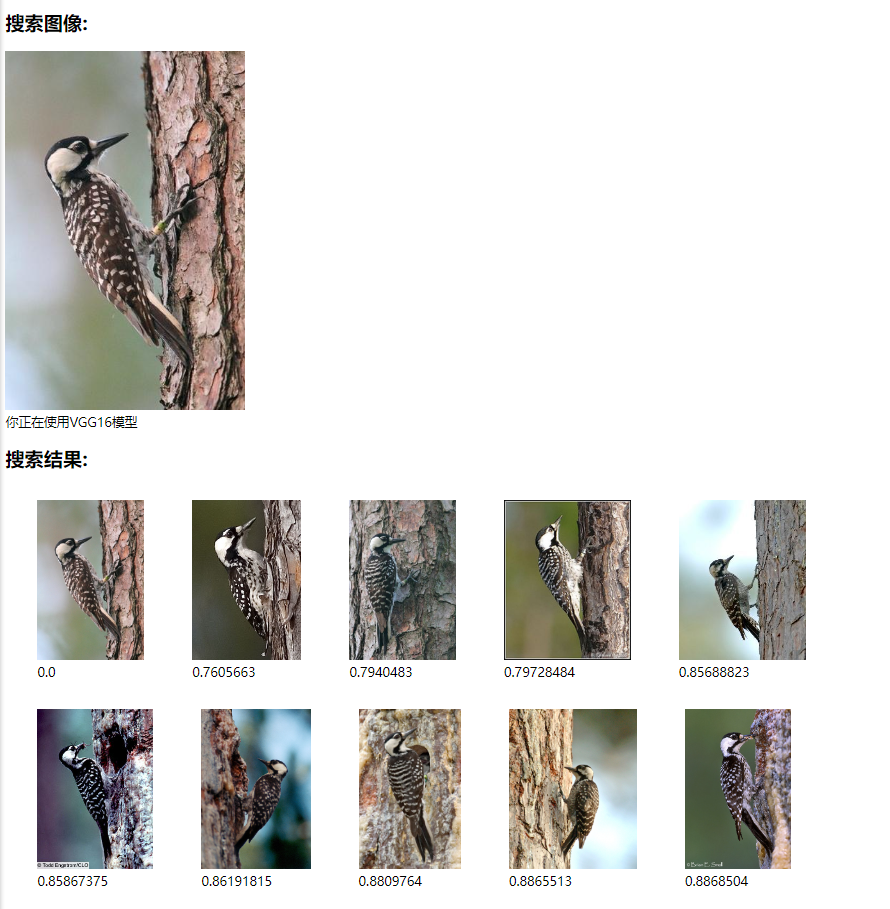
\includegraphics[width=0.9\textwidth]{PIC6}
  \caption{斑点、纹理规则鸟类.}
  \label{fig_PIC6}
\end{figure}

\begin{figure}[!htb]
  \centering
  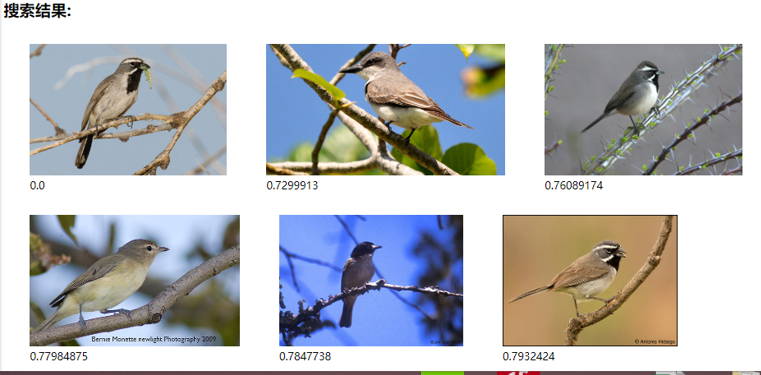
\includegraphics[width=0.6\textwidth]{PIC7}
  \caption{整体构图.}
  \label{fig_PIC7}
\end{figure}

然而要注意的是,这并不代表该图像检索引擎会忽略其他重要的特征,如整体构图等。如图3-4,虽然这次检索返回的相关图片较少,但是排行前列的图片与检索图像的背景构图相似度较高,说明该模型算法也很好的学习到了整体构图特征。

在测试中服务端的Python进程占用内存较大,约7GB,若服务端总使用内存超出单条内存的容量则有可能导致python内存溢出报错。建议运行服务器前事先用任务管理器结束其他无用的进程。服务端的CPU和GPU的负载也较高,CPU多个核心使用率达到90$\%$以上,显存也基本满载。认定是程序架构的问题,内存中加载的数据过多,python无法使用更多的内存。可以用resource库提高可使用的的内存上限,或者更改程序,降低内存一次性读取的数据量。对于性能较差的电脑建议使用轻量级的mobilenet模型。

\begin{figure}[!htb]
  \centering
  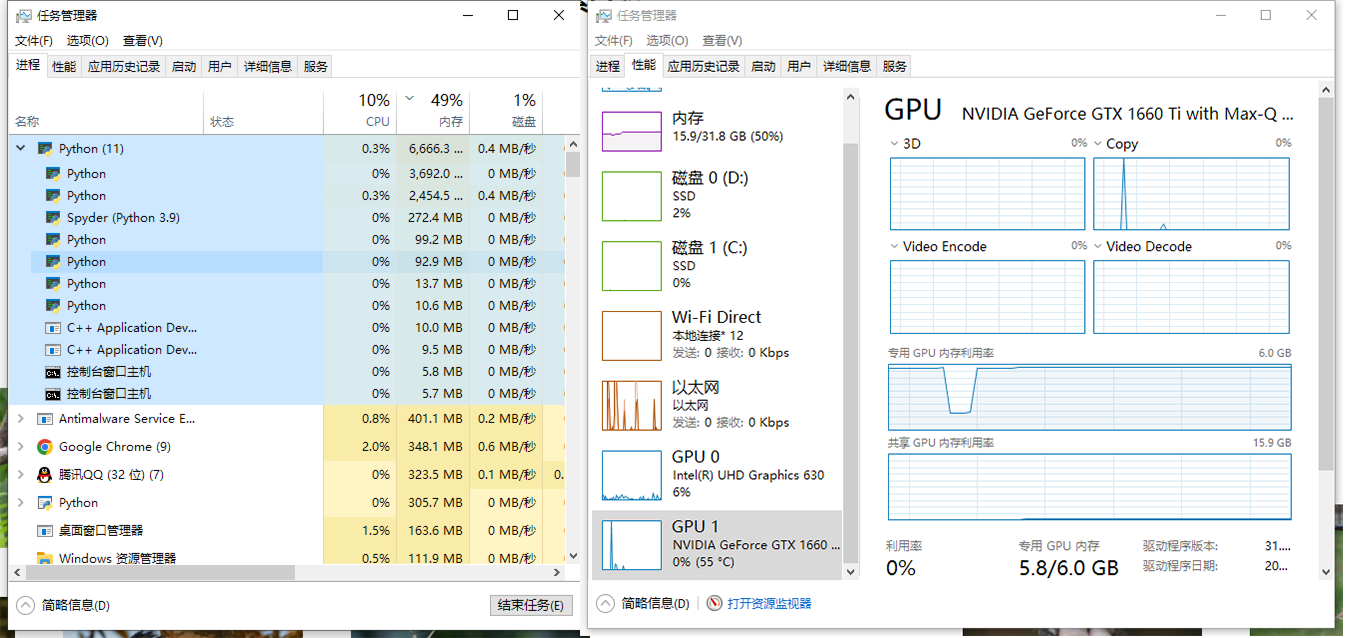
\includegraphics[width=1\textwidth]{RAM1}
  \caption{python占用.}
  \label{fig_RAM}
\end{figure}

\chapter{总结和展望}

\section{总结}

本文主要介绍了“基于Python的图像搜索引擎设计”项目的设计过程和主要内容。首先,本文介绍了图像搜索引擎的概念和发展历史,随后分析了图像搜索引擎发展的现状,分析了多种算法的优缺点。接着本文讲解了基于Python实现图像搜索引擎的具体步骤,包括特征提取、网络架构、相似度计算、用户交互界面设计等。最后本文展示了该图像搜索引擎的性能测试结果并作出了分析总结。本项目对高色差饱和度、斑点、纹理较为敏感,相关图片识别率较高。

另外还在基础的图像检索功能以外作出了扩展,比如图像标注功能、图像裁剪预处理功能和前端上传数据功能。

\section{展望}

本项目实现了一个简单的基于python的图像搜索引擎,但是本项目还存在着一些不足,例如当数据库较大时,程序容易内存溢出无法提供服务,程序特征提取较慢。对构图较复杂的核心目标识别率较差。有很多可以改进和扩展的方向。以下是我对未来工作的展望。

1.在特征提取和相似度计算方面,可以由网页端来切换模型特征输出层和相似度计算公式。例如在保持服务器运行的同时VGG16的fc1层替换为mobilenet的fc层,或将相似度计算的欧式距离换为汉明距离和余弦距离。

2.目前只支持静态图片的搜索,如何支持更多种类的数据搜索,如动图、视频等等。

3.关于网络架构的替换,flask受限于进程锁。如何将flask网络框架更换为如Quart和Sanic的异步网络框架,增强其服务器性能。

4.增加网页端用户交互性,用户在使用时可以标记、评分等,增加一些图片的权重,进一步优化嗖嗖的结果。

5.在处理大规模数据集时,如何利用分布式计算、GPU加速等加快效率、准确率,并降低服务端的负担。

6.应用到更多领域:例如农业、医疗、电商等行业。

总之,基于python的图像搜索引擎是一个具有广泛发展应用前景的技术,通过丰富且功能强大的库文件和不断地改进拓展,它将会在各个领域发挥越来越重要的作用。








%%%%%%%%%%%%%%%%%致谢%%%%%%%%%%%%%%%%%%%%%%%%%%%%%%%
 



\acknowledgement

 
在毕业设计的实践中,从对课题的了解,总体框架的建立,基本功能的实现,扩展功能思路的产生,中间有着我自己的努力,也少不了指导老师的教导。

在这里我首先要感谢相成娣老师和翁立老师,他们对我的项目提供了宝贵的指导和建议,并在项目实现过程中给予了我充分的支持和鼓励。在此我致以最诚挚的谢意!

我还要感谢一位异国的友人Yusuke Mastsui,是他解答了我困扰已久的疑惑。

我还要感谢母校和老师们四年以来对我的栽培。

同时我还要感谢所有为本项目提供数据、信息的机构和个人,没有他们的支持,本项目绝不会如此圆满完成。

在此表达深深的谢意。
%%%%%%%%%%%%%%%%%%%%%%%%%%%%%%%%%%%%%%%%



%%%%%%%%%%%%%%%%%%%%%%%%%%%%%参考文献%%%%%%%%%%%%%%%%%%%%%%%%%%%%%%%%%
\hdubibliography{ref/reference}
%\bibliographystyle{hdu-thesis}
%\bibliography{ref/reference}
% % %%%%%%%%%%%%%%%%%%%%%%%%%%%%%%%%%%%%%%%%%%%%%%%%%%%%%%%



% %%%%%%%%%%%%%%%%%%%%%%%%%%%%附录%%%%%%%%%%%%%%%%%%%%%%%%%%%%%%%
\hduappendix
项目在GitHub上的地址:https://github.com/OpoemJam/Image-search-based-on-python。其中包含了项目源文件,和一些注释,也可以通过issues提交bug。

CUB-200是一个用于鸟类识别的图像数据集,它包含了200个不同种类的鸟类,每个种类包含大约60张图像,总共有11788张图像。官方网站为:http://www.vision.caltech.edu/
datasets/cub$\_$200$\_$2011/。这个网站还包含了不少其他有研究价值的数据集。
 

%%%%%%%%%%%%%%%%%%%%%%%%%%%%%%%%%%%%%%%%%%%%%%%%%%%%%%%%%%%%



\end{document}